% find . -type f -name 'main.*' -not -name '*.tex' -not -name '*.pdf' -delete
%%%%% find . -type f -not -name '*.tex'  -newer main.tex -delete
%%%%% pandoc main.tex -o output/main.docx
%%%%% pdflatex -output-directory=output main.tex
%%% not working
% find . -type -not -name '[{tex}|{jpg}|{png}|]'
% find . -type f -not \(-name '*gz' -or -name '*tex' -or -name '*jpg' -or -name '*png' -or -name '*bib' \) -delete

%%%%%%%%%%%%%%%%% DOCUMENT TYPE DEFINITION

\documentclass[openright, a4paper, oneside, openany]{report}

%%%%%%%%%%%%%%%%% END OF DOCUMENT TYPE DEFINITION


%%%%%%%%%%%%%%%%% PACKAGES

% \usepackage[english]{babel}  % Last language is the documents standard one.
\usepackage[T1]{fontenc}
% \usepackage{book}
\usepackage{listings}
\usepackage{hyperref}
\hypersetup{colorlinks=false}
\usepackage{lscape}
\usepackage{amsmath} % Extra commands for math
\usepackage{amssymb} % Math symbols
\usepackage{graphicx}
\usepackage{subfig}
\usepackage[colorinlistoftodos]{todonotes}
\usepackage{color}
\usepackage[a4paper,top=2.54cm,bottom=2.54cm,left=3.81cm,right=2.54cm,marginparwidth=1.75cm]{geometry}
% \usepackage [ Bjornstrup ]{ fncychap }
% \usepackage{nomencl} % Nomenclature
% \makenomenclature

\usepackage{booktabs}
\usepackage{indentfirst} % Package to indent the first paragraph
\usepackage{lipsum} % Package for dummy text

\usepackage{afterpage}

\usepackage{mathptmx}
\usepackage{anyfontsize}
\usepackage{t1enc}
\usepackage{seqsplit}

\newcommand\blankpage{%
    \null
    \thispagestyle{empty}%
    \addtocounter{page}{-1}%
    \newpage}

% Glossary
\newglossaryentry{latex}
{
    name=latex,
    description={Is a mark up language specially suited for scientific documents}
}

\newglossaryentry{maths}
{
    name=mathematics,
    description={Mathematics is what mathematicians do}
}

\newglossaryentry{formula}
{
    name=formula,
    description={A mathematical expression}
}

\newacronym{gcd}{GCD}{Greatest Common Divisor}

\newacronym{lcm}{LCM}{Least Common Multiple}
%%%%%%%%%%%%%%%%% END OF PACKAGES



%%%%%%%%%%%%%%%%% PATHS

\graphicspath{{./frontmatter/images/}{./mainmatter/1-Introduction/images/}{./mainmatter/2-Development/images/}{./mainmatter/3-Methodoly/images/}{./mainmatter/4-Results/images/}{./mainmatter/5-Conclusion/images/}{./backmatter/appendix/images/}}

%%%%%%%%%%%%%%%%% END OF PATHS




%%%%%%%%%%%%%%%%% HEADINGS CONFIGURATION

\usepackage{fancyhdr}
% \pagestyle{fancy}
% \fancyhead[LE,RO]{\textsl{\rightmark}}
% \fancyhead[LO,RE]{\textsl{\leftmark}}


\renewcommand{\chaptermark}[1]{%
\markboth{\chaptername
\ \thechapter.\ #1}{}}

\renewcommand{\sectionmark}[1]{\markright{\thesection.\ #1}}

% Delete headings of blank pages

\makeatletter
\def\cleardoublepage{\clearpage\if@twoside \ifodd\c@page\else
\hbox{}
\vspace*{\fill}
%\begin{center}
%This page intentionally contains only this sentence.
%\end{center}
\vspace{\fill}
\thispagestyle{empty}
\newpage
\if@twocolumn\hbox{}\newpage\fi\fi\fi}
\makeatother

\clearpage{\pagestyle{empty}\cleardoublepage}

%%%%%%%%%%%%%%%%% END OF HEADINGS CONFIGURATION

%%%%%%%%%%%%%%%%% Caption
\usepackage{caption}

% \captionsetup{%
%   font=footnotesize,% set font size to footnotesize
%   labelfont=bf % bold label (e.g., Figure 3.2) font
% }
% \captionsetup{
%    tablename=Table,
%    listformat=empty,
%    justification=justified,
%    labelsep=quad,
%    position=above,
%    skip=\onelineskip,
%    width=\linewidth,
%    labelfont={small},
%    font={small}
% }
\usepackage{array,booktabs}
\usepackage{framed}
\usepackage{float}
\usepackage[framed,amsmath,thmmarks]{ntheorem}
\usepackage{titlesec}


%  Title Formats
\titleformat{\chapter}[hang] 
{\normalfont\huge\bfseries}{\chaptertitlename\ \thechapter:}{8pt}{} 
\titlespacing*{\chapter}{0pt}{-35pt}{20pt}
\titleformat*{\section}{\normalfont\Large\bfseries}
\titleformat*{\subsection}{\normalfont\large\bfseries}
\titleformat*{\subsubsection}{\normalfont\normalsize\bfseries}

% Clear empty pages between chapters
\let\origdoublepage\cleardoublepage
\newcommand{\clearemptydoublepage}{%
  \clearpage
  {\pagestyle{empty}\origdoublepage}%
}
\let\cleardoublepage\clearemptydoublepage

\usepackage{setspace}
% \usepackage[nottoc,notlof,notlot]{tocbibind} 
% \usepackage {tikz}
% \usetikzlibrary {positioning}
% %\usepackage {xcolor}
% \definecolor {processblue}{cmyk}{0.96,0,0,0}

% \usepackage{footnote}
% \usepackage{amsfonts}
% \usepackage{svg}

% Add figure and table
\usepackage{chngcntr}
\usepackage{wrapfig}
\usepackage{booktabs}
\captionsetup[table]{position=top}
\captionsetup[subfloat]{position=bottom}
\captionsetup[figure]{position=bottom}

% \usepackage[backend=bibtex]{biblatex}

\usepackage[english]{babel}
\newcommand{\lat}{\selectlanguage{english}}

\newcommand{\campusaddress}{Lalitpur, Nepal}

% \hyphenpenalty=100000
\DeclareUnicodeCharacter{0080}{HERE-HERE-HERE}
%%%%%%%%%%%%%%%%% PARAGRAPHS CONFIGURATION

\setlength{\parindent}{1.3cm}
\setlength{\parskip}{0.2cm}

%%%%%%%%%%%%%%%%% END OF PARAGRAPHS CONFIGURATION


%%%%%%%%%%%%%%%%% PREAMBLE


\author{Anup Adhikari}
\date{2019}

\title{Protein Drug Interaction from their sequence}
\newcommand{\mysubtitle}{Using the SMILES and SEQUENCE information}
\newcommand{\mygrade}{Electrical Engineering}
\newcommand{\myuniversity}{Tribhuwan University}
\newcommand{\myinstitute}{Institute of Engineering}
\newcommand{\mydepartment}{Department of Electronics and Computer Engineering}
\newcommand{\mycampus}{Pulchowk Campus}
\newcommand{\myadvisorA}{Dr. Surendra Shrestha}
%\newcommand{\myadvisorB}{Department Bertan of Electrical Engineering}
%\newcommand{\myadvisorC}{Department Bertan of Electrical Engineering}

\newcommand{\roll}{073 MSCS 652}
\makeatletter
\let\thetitle\@title
\let\theauthor\@author
\let\thedate\@date
\makeatother

%%%%%%%%%%%%%%%%% END OF PREAMBLE

\newcommand{\rowstyle}[1]{\gdef\currentrowstyle{#1}%
  #1\ignorespaces
}


%%%%%%%%%%%%%%%%% MAIN DOCUMENT

\begin{document}

\frenchspacing

% Frontmatter

%\input{frontmatter/1-coverpage.tex}
%\begin{titlepage}
\begin{center}
    
	\begin{minipage}{0.48\textwidth} \begin{flushleft}
    \includegraphics[height = 2.5cm]{frontmatter/images/logo1.PNG}
    \end{flushleft}\end{minipage}
    \begin{minipage}{0.48\textwidth} \begin{flushright}
    \includegraphics[height = 2.5cm]{frontmatter/images/logo2.PNG}
     \end{flushright}\end{minipage}
     
    \vspace*{1.5cm}

    \textsc{\LARGE \myuniversity}\\[0.2cm]
    \textsc{\large \myschool}\\[1.5cm]
    
    
    \vspace*{1cm}

  { \huge \bfseries \thetitle }\\[0.4cm]	
    \vspace*{2cm}
  
  { \large 
    \emph{Student:} \\	
      \theauthor \\
    \vspace*{0.5cm}
    \emph{Academic Advisers:} \\													  
      \myadvisorA \\
      Advisor 2	\\
    \vspace*{0.5cm}
    \emph{Company Advisers:} \\													  
      Advisor 1 \\
      Advisor 2	\\
  }

  \vspace{2cm}
    Final project report for the \mygrade \: graduation.	\\	

  \vspace{3cm} 	
  \begin{center}
    {\thedate}
  \end{center}
 
    
\end{center}
\end{titlepage}
\begin{titlepage}

\begin{center}

\includegraphics[height = 2.6cm]{frontmatter/images/tu.jpg} 

\linespread{1.5}

\bf{
    \vspace{0.5cm}

\MakeUppercase{\myuniversity}
    % \vspace{0.3cm}

\MakeUppercase{\myinstitute}

\MakeUppercase{\mycampus }

% \MakeUppercase{ \campusaddress}
\vspace{1cm}

\begin{flushleft}
   \MakeUppercase{thesis no.: \roll } 

   
\end{flushleft}

{\thetitle}
% \mysubtitle

% \vspace{1cm}

% {\lat \large{\thetitle}}\\



\vspace{1cm}
{by}
 
\theauthor

\vspace{1cm}

% {Supervisor} \\
% \myadvisorA

\vspace{1cm}

% {\em This Thesis is carried out as a part of the education at the \myuniversity \: and is therefore approved as a part of this education. However, this does not imply that the University answers for the methods that are used or the conclusions that are drawn.}
{A THESIS  

SUBMITTED TO THE DEPARTMENT OF ELECTRONICS AND
COMPUTER ENGINEERING 

IN PARTIAL FULFILLMENT OF THE REQUIREMENT FOR THE 

DEGREE OF MASTER OF SCIENCE IN COMPUTER SCIENCE AND KNOWLEDGE ENGINEERING
}
\vspace{1cm}

\MakeUppercase{\mydepartment}

\MakeUppercase{\campusaddress}

\vspace{1cm}

NOVEMBER,
\thedate
% \myuniversity, \thedate \\
% \myinstitute \\
% \mycampus \\
% \mydepartment
}
\end{center}
 % Bold Faced
\end{titlepage}

\cleardoublepage
\setcounter{page}{1}
\linespread{2}
\doublespacing


\chapter*{Recommendation}
\vspace{3cm}
The undersigned certify that they have read and recommended to the Department of Electronics and Computer Engineering for acceptance, a thesis entitled “\textit{\thetitle}”, submitted by \theauthor in partial fulfillment of the requirement for the award of the degree of “Master of Science in Computer System and Knowledge Engineering.

\vspace{3cm}
..........................................

Supervisor

Dr. Surendra Shrestha (PhD)

\vspace{3cm}


..........................................

External Examiner

Name:









\chapter*{Departmental Acceptance}

\textit{(Use letter department’s letter pad for this page)}
\vspace{3cm}

The thesis entitled "\thetitle", submitted by \theauthor in partial fulfillment of the requirement for the award of the degree of “Master of Science in Computer System and Knowledge Engineering” has been accepted as a bonafide record of work independently carried out by him in the department.





\vspace{3cm}
. . . . . . . . . . . . . . . . . . . . . . . . . . . . . . . . . . . . . . . . . . . 

Dr. Surendra Shrestha (PhD)

Head of the Department

Department of Electronics and Computer Engineering,

Pulchowk Campus,

Institute of Engineering,

Tribhuvan University,

Nepal.


%\selectlanguage{english}
%\begin{abstract}
%\end{abstract}

%\selectlanguage{french}
%\begin{abstract}
%\end{abstract}

\chapter*{Abstract}
\doublespacing
Protein and Drugs are the major analysis subjects in computational bioinformatics to produce conclusions in treatment of diseases. While scientific methods are progressing with experiments and medical principles, they are still expensive means to discover the cure of new diseases. In principle, the high computing systems can be used to reduce the costs related to discovery. With the evolving nature of disease for instance, due to mutation, there has been extensive research work on exploring the fundamental properties of proteins and drugs to find the correct match in treatment. Finding the interaction between drugs and proteins based on their molecular fingerprints and protein sequences has been explored using statistical methods and rule-based methods. The representation of drugs in fingerprints and proteins in sequence are used to map them to different domains, which are then trained in a deep neural net to produce a regression solution. Instead of relying on binary classification, the more superior KIBA scores are used to quantify the interaction score between the drugs and proteins. The feature vectors, PSSMDT, Embedding and RPT, are combined to aid the deep learning state-of-art solution with convolution and dense layers, and aid to prediction score of 89\%.
\chapter*{Acknowledgement}


I would like to express the deepest appreciation to my supervisor and Head of Department of Electronics and Computer Engineering, Pulchowk Campus \myadvisorA for his guidance throughout the period of this work. His invaluable support, understanding and expertise have been very important in completing this work. It was a great honor for me to pursue my thesis under his supervision.

I pay my sincere gratitude Dr. Aman Shakya, to MSCSKE Coordinator for his supervision and help during this research work.

I am highly grateful to Prof. Dr. Shashidhar Ram Joshi, Prof. Dr. Subarna Shakya, Dr. Sanjeeb Prasad Pandey, Dr. Dibakar Raj Pant and Dr. Basanta Joshi for their encouragement and guidance.

I would like to express my heartily gratitude towards the \myinstitute, \mycampus along with all my respected teachers, my friends, my family for giving me continuous support for their invaluable help.


{\bf{\theauthor}}


{\bf{\roll}}


{\bf{\myinstitute}}


%\renewcommand{\abstractname}{Remerciements}
%\begin{abstract}
%\end{abstract} 


\tableofcontents
\listoffigures
\listoftables

% \printnomenclature

% \newcommand{\listequationsname}{List of Equations}
% \newlistof{myequations}{equ}{\listequationsname}
% \newcommand{\myequations}[1]{%
% \addcontentsline{equ}{myequations}{\protect\numberline{\theequation}#1}\par}
% \setlength{\cftmyequationsnumwidth}{2.5em}% Width of equation number in List of Equations
% \listofmyequations
% Mainmatter




\setcounter{page}{1}
\chapter{Introduction}
\section{Background}
Treatment of diseases are mostly associated with applying foreign medicinal components into human body. The rudimentary means of curing diseases has been growing with applied ayurbedas since the past. The chemical perspective of curing diseases slowly evolved into modern chemistry as drug facilities developed around the globe. The extensive research and documentation changed the world where people have come to trust fully in chemist's drugs to mitigate the ailments in the body. With the growing chemical interest in the community, the need to develop better drugs and quick solutions increased even higher. With the identification of new diseases and dire need of understanding the mechanism to cure such diseases, the drug research started gaining its speed.

~\acrfull{cadd} mechanism have been developing in bio-informatics ever since the "Next Industrial Revolution" possibilities started grow~\citep{Leelananda2016,Brown2017}. The interest started as Fortune magazine published the article "Designing Drugs by Computer at Merk". Experimenting with computational power and technical human resources in biomedicine, the concepts started to form scopes like \acrfull{hts} -- A technique to screen desired drugs from other drugs. \acrshort{hts} was evolving eventually to find precedence over finding novel therapeutics. The desire to increase high hit rate did grow as the traditional \acrshort{hts} led to few probable leads. As research developed on computational drug design, \acrshort{cadd} study broadened based on the computational resources required. ~\acrshort{cadd} can be classified into two general categories: Structure-based \acrshort{cadd} and Ligand-based~\acrshort{cadd}.

Structure based \acrshort{cadd} relies on knowledge of structural analysis of protein structures in particular to identify the drug leads. It associates to phenomenons like Binding Site Analyses, Docking Simulations, and Scoring Algorithms. In brief, all the structural properties of proteins are exploited to identify the possible drug candidates -- the molecules which fit in the protein structure description. This work borrows the representational feature sets of proteins and drugs from this discipline.

%Target Structure Preparation, binding site detection, representation for docking simulations, scoring functions, sampling algorithms for docking,HTS, Site Characterization, Parmacophore model.  
 
Ligand-based \acrshort{cadd} exploits similarities of known active and inactive molecules. It further exploits the chemical, electrical and functional properties from drugs and proteins. This work borrows the feature representations of chemical-electrical properties in the form of \acrfull{srv}.

%Descriptors, Similarity Search Molecular, QSAR model, Pharmacophore, Prediction to Optimization

This work relates mostly to the Structure based \acrshort{cadd} and partly to Ligand-based \acrshort{cadd}. 
\iffalse
The parameters of our work can be associated with \begin{itemize}
    \setlength\parindent{24pt}
    \item Target Structure %, De novo design 
    \item Ligand Structure %, Ligand based virtual screening
\end{itemize}
\fi
Target Structure and Ligand Structures are the major parameters of the research. The de-novo design has not been explored yet but the research method in this work can be used to test the drug designs for Structure Generator\footnote{Structure Generator: The molecules which are highly active, readily synthesizable and devoid of undesirable properties are used to construct new possible drugs and can be tested with multiple targets.}. The other aspects of target identification -- Molecular Dynamics, Pharmacophore modeling, Ligand Docking, \acrfull{qsar} etc. are beyond the scope of this work. So, the predictions from the model may not be sufficient to conclude the predicted interaction results. The pharmacophore models could take the results from this work and make decisive conclusions. 

\iffalse
(52498, 254)
180244
\fi
The Dataset contains scores of the interaction of proteins and drugs based on \acrshort{kiba} scores. We use \arabic{no_drugs} drugs from CHEMBL and \arabic{no_proteins} proteins from UniProt to get their structural information. The interaction of 180244 is obtained from the research work produced by \citep{Tang2013}, and by removing the unrecognized interactions. The interactions are based on KIBA score -- an integrated approach by combining the power of thermodynamic constants and activity percentage of drug-target interaction profile.

\iffalse

For citations, use the function \textbackslash cite. \citep{gowar1989power} The references file is the sample.bib one. Google Scholar provides almost all the references in LaTeX form.

To insert a footnote, use the following command. \footnote{This is a footnote.} When necessary to use a nomenclature, define it on the same page for a better organization. Don't create NSN (Non-sense nomenclatures).

For figures, tables, equations and further information, open the file "tips.tex". If what you need is not found there, Google it.

% Add nomenclature at each new used nomenclature
\fi
 
\section{Statement of Problem}
The simple technique of encoding the sequence information of drugs and proteins to identify if a drug will interact with the protein or not has a major issue. While drugs encoding information can be used to make drug related predictions, the protein encodings require additional feature vector input to properly form their representational vectors. For instance, the docking of drugs to protein structure doesn't only depend on surface area, a condition that structural representation can learn with proper algorithm, but also with electric field and H-bond properties \citep{Wong2018}. Therefore, modeling a machine learning algorithm sometimes overfit the situation or poorly classify the problem. In this work, we explore various features integration like R2RSRV and PSSM matrix along with sequence feature set and reproduce a regression problem for solving the prediction problem.

\subsection{Selection of Prediction Score}

The research explored different score functions used to predict the interaction of drug and protein. Among STITCH, Davis, Metz\_Anastassiadis and KIBA scores, KIBA scores were used for the prediction of drug and protein interaction problem. The main reasons are: STITCH scores don't fully explore the primary thermodynamic dissociation constants used for drug-target interaction profile. The information of other scores are present in KIBA~\citep{Tang2013}, as shown in section~\ref{section:kiba}. Again, KIBA scores dataset is sourced from multiple databases \citep{Kanehisa2000}, \citep{Wishart2018}, \citep{Hecker2012} and \citep{Sharma2010} a consists of experimental data and secondary data (from literature) of drug-target interaction. Choosing the KIBA as the output score for two protein and drug sequences, we model our machine learning algorithm for prediction of interaction.

\subsection{Selection of Features}

For the protein family, the focus here is with the kinase target family because of their essential roles in cellular signaling transduction for many cancers and inflammatory diseases~\citep{Tang2013,Kanehisa2000}. We concentrate on proteins dataset, specifically because their interaction is quite tricky when considered among chemical, atomic, structural and electrical nature of protein residues~\citep{Mathai2019}. Our basis for forming the matrices and vectors related to protein sequence came from the fact that these features represent specific properties related to the protein and its residues. Also, the literatures describing the feature sets characteristics and results motivates us towards the selection of these parameters: labeled encodings, \acrshort{pssmdt}, \acrshort{edt} and \acrshort{rpt}.


\section{Objectives}
The objectives of the research are:
\begin{itemize}
    \setlength\parindent{36pt}
    \item To determine the effective feature matrices related to protein.
    \item To modify DeepDTA - a deep learning architecture using \acrfull{cnn} for predicting the protein-drug interactions.
\end{itemize}

\section{Scope of Work}


\subsection{Choosing Method of Interaction}
The work explored two popular techniques used in prediction problem: Global Methods and Local Methods. Global Method tries to predict the label of one residue pair considering the label of others while Local Method tries to predict the label of one residue pair without considering the label of others. The work used Global Methods as a means of protein-drug interaction prediction. It tried to run different variations in Residual Methods: Using Distance Prediction, Coevolutionary features, Sequence Representation. 

\iffalse
\subsection{Creating Analogy with Image}
For any protein sequence, instead of regarding them as segments, we try to run the whole protein sequence as an image: the residual contacts representing the pixels of the image.
\fi

\subsection{Deep Learning Network Selection}
Convnets, as they still are quite helpful in solving an image recognition problem, we used the stack of CNN with other keras layers to understand the performance of prediction of interaction with protein drug set. The image problem is in analogy as the different canonical dimension of drugs being mapped with canonical dimension of proteins. The value of pixel can be thought of as an interaction value of drug substituent with protein substituent.

\subsection{Training and Testing}
A basic PC was used to create initial models. Google Colabs was used to train the deep convolutionary stack due to requirement of GPU. The models were saved on the runtime so that the next training could be resumed immediately after the cease of Colab's VM Session.

\section{Organization of Thesis}

{{\uppercase{\bf{Chapter 1}}}
is the introductory chapter that includes background of the study, problem statement, objectives of thesis and scope of the work.
}

{{\uppercase{\bf{Chapter 2}}}
    is the literature review about the work. It describes No Free Lunch Algorithm and Generalized Optimization; their concepts and implications to this work. The build up describes how the various literatures assist to provide motivation to this work.
}

{{\uppercase{\bf{Chapter 3}}}
  describes details of Methodology used for Protein and Drug Interaction prediction problem. The system block of \acrfull{featdti} is described. The properties of data used for training the model are described. It underlines the principles on \acrfull{pssm}, \acrfull{pssmdt}, \acrfull{edt}, \acrfull{rpt}, and labeled encodings used for feeding the Deep Learning Network. The components of \acrfull{featdti} used as deep learning model in this work are described.
}

{{\uppercase{\bf{Chapter 4}}}
    describes the experimental settings and results produced in this work. The analysis of work produced is described in detail.
}

{{\uppercase{\bf{Chapter 5 and Chapter 6}}}
    describe the conclusions from the work and recommendations for future work. 
}

{{\uppercase{\bf{Appendix}}}
     enlists the data parameters used in the work and describes their integration in this work.
}

{{\uppercase{\bf{References}}}
    enlists the references used for this thesis completion.
}
\chapter{Theorical Background}


\section{No Free Lunch Algorithm}

\lipsum[2-3]

\section{Stacking Generalization}

\lipsum[2-3]

\section{Literature Review}

\lipsum[2-3]
\iffalse

% curl http://ulms2019.nsdevil.com:10002/edit/lms/self/data/original_kiba/figures.zip -o /anup_files/FILES/personal/Thesis/mainmatter/3-Methodology/images/figures.zip; % login error so file not downloaded
% mv ~/Downloads/figures.zip /anup_files/FILES/personal/Thesis/mainmatter/3-Methodology/images/figures.zip;
% unzip /anup_files/FILES/personal/Thesis/mainmatter/3-Methodology/images/figures.zip -d "/anup_files/FILES/personal/Thesis/mainmatter/3-Methodology/images/"; 
% rm /anup_files/FILES/personal/Thesis/mainmatter/3-Methodology/images/figures.zip


Statistical Analyses to DO:
1. KIBA Score Distribution
2. Amino Acid counts (20 standards) -- For each protein sequence get total counts, sort by length -- (corresponding to one-hot)
3. Drug Sequence Counts similar to amino acid (Logarithmic-corresponding to one-hots)
4. 
Things to do:
1. System Block remake (remove calculation of KIBA Scores)
\fi \usetikzlibrary{arrows,automata}
\chapter{Methodology}

\section{System Overview}

\subsection{System Block}

\begin{figure}[H]
  % \def\svgwidth{\columnwidth}
  % \includesvg{mainmatter/3-Methodology/images/block.svg}
  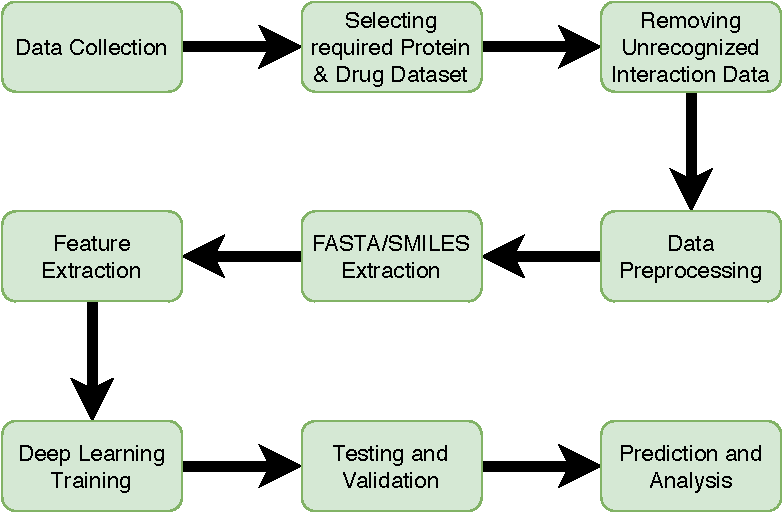
\includegraphics[width=1\linewidth]{mainmatter/3-Methodology/images/system_block.pdf}
  \caption{System Block Diagram for Protein-Drug Prediction}
  \label{fig:system}
\end{figure}

Figure ~\ref{fig:system} shows the different stages of research for building a protein drug prediction system. The data is collected by exploring the available internet sources and required dataset is downloaded for processing. From the data, the missing values are removed in data preprocessing to aid proper training. From the raw drugs and proteins profile, SMILES and FASTA sequences are extracted respectively. Now the features are extracted based on the sequence provided. Then, the features are fed into Deep Learning Algorithm where the training is performed to create the right prediction system. The training follows by testing and validation of data under different settings of protein and drug combinations.


\subsection{Data Collection}

The dataset is collected from open-internet database. Basically, there are three types of data required in this work: protein, drug and interaction sets. The UniProt Library has been used for extracting proteins features, PubChem for drug features, and NCBI for interaction scores. Additionally, PSI-BLAST is used to generate PSSM matrices for the protein features downloaded.

UniProt contains database of 173,281 proteins of human (Homo sapiens) (until 2019). The protein document consists of the taxonomic classification, identifiers to other databases for cross-linking,  molecular properties, related specific bioactivity, functional property, canonical and isoforms of protein sequence. The protein fasta sequence in particular is of interest to this research. An API can be used to download the available information.  
\url{https://www.uniprot.org/help/programmatic_access}

>O00311

\seqsplit{MEASLGIQMDEPMAFSPQRDRFQAEGSLKKNEQNFKLAGVKKDIEKLYEAVPQLSNVFKIEDKIGEGTFSSVYLATAQLQVGPEEKIALKHLIPTSHPIRIAAELQCLTVAGGQDNVMGVKYCFRKNDHVVIAMPYLEHESFLDILNSLSFQEVREYMLNLFKALKRIHQFGIVHRDVKPSNFLYNRRLKKYALVDFGLAQGTHDTKIELLKFVQSEAQQERCSQNKSHIITGNKIPLSGPVPKELDQQSTTKASVKRPYTNAQIQIKQGKDGKEGSVGLSVQRSVFGERNFNIHSSISHESPAVKLMKQSKTVDVLSRKLATKKKAISTKVMNSAVMRKTASSCPASLTCDCYATDKVCSICLSRRQQVAPRAGTPGFRAPEVLTKCPNQTTAIDMWSAGVIFLSLLSGRYPFYKASDDLTALAQIMTIRGSRETIQAAKTFGKSILCSKEVPAQDLRKLCERLRGMDSSTPKLTSDIQGHASHQPAISEKTDHKASCLVQTPPGQYSGNSFKKGDSNSCEHCFDEYNTNLEGWNEVPDEAYDLLDKLLDLNPASRITAEEALLHPFFKDMSL}

PubCHEM and CHEMBL are drug databases used for feature extraction of drug molecules. PubCHEM is a database containing 96,881,514 drug compounds and associates to each using CID identifier. It allows programmatic access and downloads of database text files. The SMILES structure provided by the PubChem library is used to generate features corresponding to each drug molecule. The properties associated with the molecule is explored using CHEMBL database using a programmatic api request provided. 

\url{https://pubchemdocs.ncbi.nlm.nih.gov/programmatic-access}, 
\url{https://chembl.gitbook.io/chembl-interface-documentation/web-services}. 

\iffalse
UniCHEM is a very useful repository that has been integrated with various web-services. The queries can be done from GET request and JSON text can be retrieved in response to the request. The database can be used to retrieve structure information, mappings, InChIKey and source information related to drug molecule. The InChIKey is used in this work to construct features for small drug molecule (aka ligand).   
\url{https://www.ebi.ac.uk/unichem/rest}
\fi

CHEMBL379218

PubCHEM CID 11314340

\seqsplit{CC1=C2C=C(C=CC2=NN1)C3=CC(=CN=C3)OCC(CC4=CC=CC=C4)N}



For the drug-target interaction (i.e. drug-protein interaction), KIBA scores were used \cite{Tang2013} instead of binary classification. Thus, a regression model was used to predict the drug and protein interaction. The KIBA score regression has two major advantages over binary classification: interaction strength of similarly interacting ligands-target (drugs-protein) can be compared and the bias problem of unknown interactions is refrained \cite{Tang2013,ozturk2018deepdta}. Higher score means that there is more strength of interaction between the two. We use \arabic{no_drugs} ligands as drugs and \arabic{no_proteins} human proteins as target for the prediction problem.

\begin{table}[H]
  \centering
  \caption{KIBA Score Table}
  \begin{tabular}{|l|l|l|l|l|}
    \hline
   
   & O00238 & O00311 & O00329 & O00418  \\ \hline
  CHEMBL10 & 3.518514 & 3.100002 & 4.0 & 3.6  \\ \hline
  CHEMBL102000 & NaN & NaN & NaN & NaN  \\ 
  \hline
  
  \end{tabular}
  \end{table}


Various components were used to form the prediction system. Protein interaction depends on its structural, chemical, molecular(related to H-bond) and electrostatic properties. The structural representation form basis for creating features in other properties. The primary canonical structure of protein-drug set are fed into interaction block. The interaction parameter is filtered accordingly to the filter type. Similarly, the drug feature set are created to be trained with the machine learning algorithm. Finally, after training the training dataset, cross validation of the model was done.

\section{Building Components of Features Processing}
\begin{figure}[H]\centering
  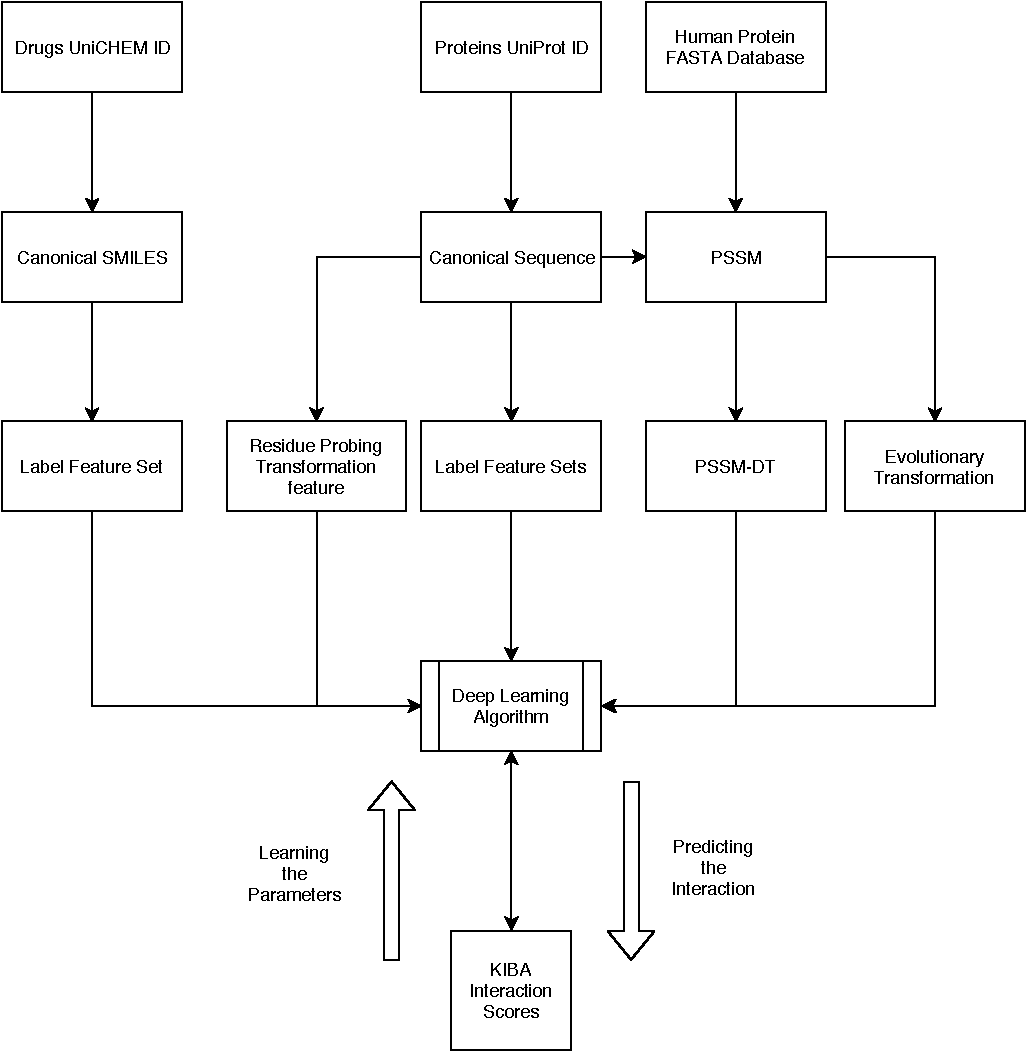
\includegraphics[width=0.9\linewidth]{mainmatter/3-Methodology/images/Algorithm.pdf}
  \caption{Schematic Block Diagram for Protein-Drug Prediction}
  \label{fig:system2}
\end{figure}

Figure \ref{fig:system2} shows the building components of the Input Vectors for feeding the deep learning network. The KIBA Prediction id done by feeding canonical protein fasta and drug smiles. The other features are constructed on their basis. PSSM matrix is constructed using PSSM matrices of human genome protein library from UniProt~\cite{UniProtConsortium2018} and the protein's FASTA. Two features, \acrfull{et} and \acrfull{pssmdt} are extracted from PSSM. From FASTA, Labelled encodings and \acrfull{rpt} matrix are created. From the SMILES, only labelled encodings is extracted.


  \section{System Block}

\begin{figure}[h]
  % \def\svgwidth{\columnwidth}
  % \includesvg{mainmatter/3-Methodology/images/block.svg}
  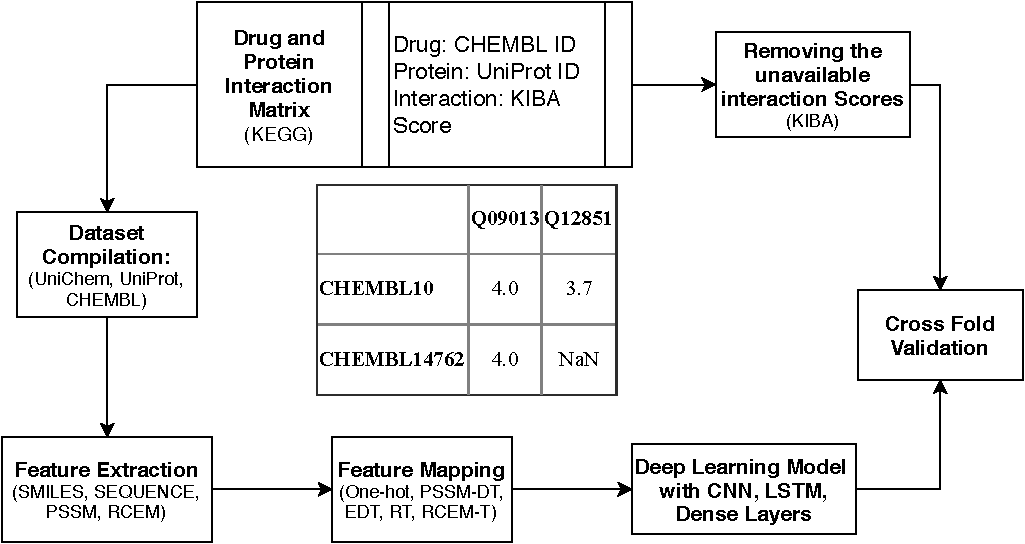
\includegraphics[width=1\linewidth]{mainmatter/3-Methodology/images/block.pdf}
  \caption{Schematic Block Diagram for Protein-Drug Prediction}
  \label{fig:system}
\end{figure}

The Figure ~\ref{fig:system} shows the various components used to form the prediction system. The idea is basic in that protein interaction depends on the structural and chemical properties. The primary canonical structure of protein-drug set are fed into interaction block. The interaction parameter is filtered accordingly to the filter type. Similarly, the drug feature set are created to be trained with the machine learning algorithm. Finally, after training the training dataset, we cross validate the model with test dataset.


\section{Dataset Description}

\iffalse
\subsection{\acrfull{kegg}}
\acrfull{kegg} is a community-driven database which contains large-scale molecular datasets generated by genome sequencing and high-throughput experimental techniuqe.\cite{Kanehisa2000, ozturk2018deepdta} We use \acrshort{kegg} DRUG dataset for finding the interaction set between DRUG and PROTEIN. The interaction score is :
\fi

\subsection{\acrfull{kiba}}
The \acrfull{kiba} Scores are collected from the publicly made available dataset \cite[\textit{Tang. et al.}]{Tang2013}. The scores are actually based on thermodynamic constants K\textsubscript{i} and K\textsubscript{d} and, remaining enzyme activity(Activity \% --  IC\textsubscript{50}) .

% \begin{flushright}
\begin{equation}
  KIBA = \begin{cases}
    K_i . {adj} & \quad {if} \; {IC_{50}\: and\, K_i \,are\, present} \\
    K_b.{adj} & \quad {if}  {IC_{50} \, and \, K_d \, are \, present} \\
    \frac{K_i . {adj} \; K_b.{adj}}{2} & \quad {if\, IC_{50}\,,K_i\, and \,K_d\, are\, present}
  \end{cases}
   \label{eq:kiba}
\end{equation}
where,
\begin{equation}
K_i.{adj} = \frac{IC_{50}}{1 + L_i(IC_{50}/K_i)}
\label{eq:ki_adj}
\end{equation}

\begin{equation}
K_d.{adj} = \frac{IC_{50}}{1 + L_d(IC_{50}/K_d)}
\end{equation}
where L\textsubscript{d} and L\textsubscript{i} are parameters defining weights of IC\textsubscript{50} in model adjustments for K\textsubscript{i} and K\textsubscript{b} 
% \end{flushright}

For a kinase inhibitor drug−target interaction, we consider the medians of three major bioactivity types IC\textsubscript{50}, K\textsubscript{i}, K\textsubscript{d} where
IC\textsubscript{50} \cite{Tang2013} is the concentration at which the inhibitor causes a 50\% inhibition of enzymatic activity and K\textsubscript{i} is defined by \begin{equation}
    Ki = \frac{IC_{50}} {1 + [S]  K_m}
    \label{eq:ki}
\end{equation} 
where,  [{S}] is the experimental substrate concentration and K\textsubscript{m} is the concentration of the substrate.

\iffalse
\begin{equation}
    \tau= \frac{(a−b)}{n(n − 1)/2}   
    \label{eq:tau}
  \end{equation}
  { Here {a} and {b} represent the number of concordant pairs and discordant pairs respectively. }
\fi


All the bioactivity types are available from CHEMBL\cite{Gaulton2017}. Based on interaction data available, we remove the unknown values and get a total of 180244 interaction KIBA score values in the range of -3.09 to 17.8. With the standard deviation of 1.22, it represents a total of \arabic{no_proteins} proteins and \arabic{no_drugs} drugs.

\subsection{Position Specific Score Matrix}

\acrfull{pssm} is a very useful protein feature. The protein feature represented by PSSM depends on the sequence of all the proteins in consideration. The HUMAN genome protein (a database of more than 100,000) is downloaded from UniProt Library. The PSSM matrix is constructed for each of the kinase proteins based on this HUMAN Genome Protein Database. With this, the PSSM matrix is characterized according to human proteins to anticipate the prediction of new identified kinase proteins.

\begin{table}
  \centering
  {\caption{PSSM Analysis Design}
  \label{table:PSSM_Analysis} }
    \subfloat[][Protein FASTA Sequence]{
      \label{table:PSSM_Analysis:fasta} 
      \begin{tabular}{|l|l|} \toprule
      \hline
      1 & GAGGTAAAC \\ \hline
      2 & TCCGTAAGT \\ \hline
      3 & CAGGTTGGA \\ \hline
      4 & ACAGTCAGT \\ \hline
      5 & TAGGTCATT \\ \hline
      6 & TAGGTACTG \\ \hline
      7 & ATGGTAACT \\ \hline
      8 & CAGGTATAC \\ \hline
      9 & TGTGTGAGT \\ \hline
      10 & AAGGTAAGT \\ \hline
      
      \end{tabular}
    }
    \subfloat[][Frequency Table]{
      \label{table:PSSM_Analysis:frequency}
      \begin{tabular}{|l|l|l|l|l|l|l|l|l|l|} \toprule
        \hline
        
         & 1 & 2 & 3 & 4 & 5 & 6 & 7 & 8 & 9 \\ \hline
        A & 3 & 6 & 1 & 0 & 0 & 6 & 7 & 2 & 1 \\ \hline
        C & 2 & 2 & 1 & 0 & 0 & 2 & 1 & 1 & 2 \\ \hline
        G & 1 & 1 & 7 & 10 & 0 & 1 & 1 & 5 & 1 \\ \hline
        T & 4 & 1 & 1 & 0 & 10 & 1 & 1 & 2 & 6 \\ \hline
        
        \end{tabular}

    } 
  
  
  \subfloat[][Log-Likelihood Matrix]{
    % \rule{4cm}{0cm}
    \begin{tabular}{|l|l|l|l|l|l|l|l|l|l|} \toprule
      \hline 
  
          & 1 & 2 & 3 & 4 & 5 & 6 & 7 & 8 & 9 \\ \hline
      A & 0.3 & 0.6 & 0.1 & 0.00 & 0.00 & 0.6 & 0.7 & 0.2 & 0.1 \\ \hline
      C & 0.2 & 0.2 & 0.1 & 0.00 & 0.00 & 0.2 & 0.1 & 0.1 & 0.2 \\ \hline
      G & 0.1 & 0.1 & 0.7 & 1.00 & 0.00 & 0.1 & 0.1 & 0.5 & 0.1 \\ \hline
      T & 0.4 & 0.1 & 0.1 & 0.00 & 1.00 & 0.1 & 0.1 & 0.2 & 0.6 \\ \hline
      
      \end{tabular}  
      \label{table:log_likelihood_pssm}
    }
    
  
  \subfloat[][Sliding Window Score Calculation]{
    \centering
    \begin{tabular}{|l|l|l|l|l|l|l|l|l|l|}
    \hline 
    
        & 1 & 2 & 3 & 4 & 5 & 6 & 7 & 8 & 9 \\ \hline
    A & 0.3 &  &  &  &  &  & 0.7 &  &  \\ \hline
    C &  &  & 0.1 & 0.00 & 0.00 & 0.20 &  &  & 0.2 \\ \hline
    G &  & 0.1 &  &  &  &  &  & 0.5 &  \\ \hline
    T &  &  &  &  &  &  &  &  &  \\ \hline
    
    \end{tabular}  
    \label{table:motif_movement}
    }

    
    \subfloat[][Score of sliding window motifs]{
    \label{wrapTable:pssm-score}
    \begin{tabular}{|l|l|l|l|l|l|l|l|l|l|}
      \hline
      0 & 1 & 2 & 3 & 4 & 5 & 6 & 7 & 8 & 9 \\ \hline
      1.099 & 1 & 2.2 & 2.1 & 2.1 & 1.300 & 1.3 & 1.4 & 2 & 2.9 \\ \hline
      \end{tabular}
    }
\end{table}

Table \ref{table:PSSM_Analysis} shows a conventional process of calculating PSSM score values. The sequence following shows the process of calculating the scores once the PSSM distribution of the whole family is calculated. Table \ref{table:motif_movement} shows the score distribution of lowercase amino acid sequence (starting after 4th position) determined by the size of the sliding window.

\seqsplit{ACTC\textbf{agccccagc}GGAGGTGAAGGACGTCCTTCCCCAGGAGCCGGTGAGAAGCGCAGTCGGGGGCACGGGGATGAGCTCAGGGGCCTCTAGAAAGATGTAGCTGGGACCTCGGGAAGCCCTGGCCTCCAGGTAGTCTCAGGAGAGCTACTCAGGGTCGGGCTTGGGGAGAGGAGGAGCGGGGGTGAGGCCAGCAGCA} 

% % \begin{wraptable}{br}{5.5cm}
% \begin{table}[H]
%     \centering
    
% \end{table}
% % \end{wraptable}

.3, .1, .1, 0, 0, .2, .7, .5, .2  == Sum(2.1) - posix(4) -- See table \ref{wrapTable:pssm-score}

\begin{figure}[htbp]
    \centering 
          %  \subfloat[]{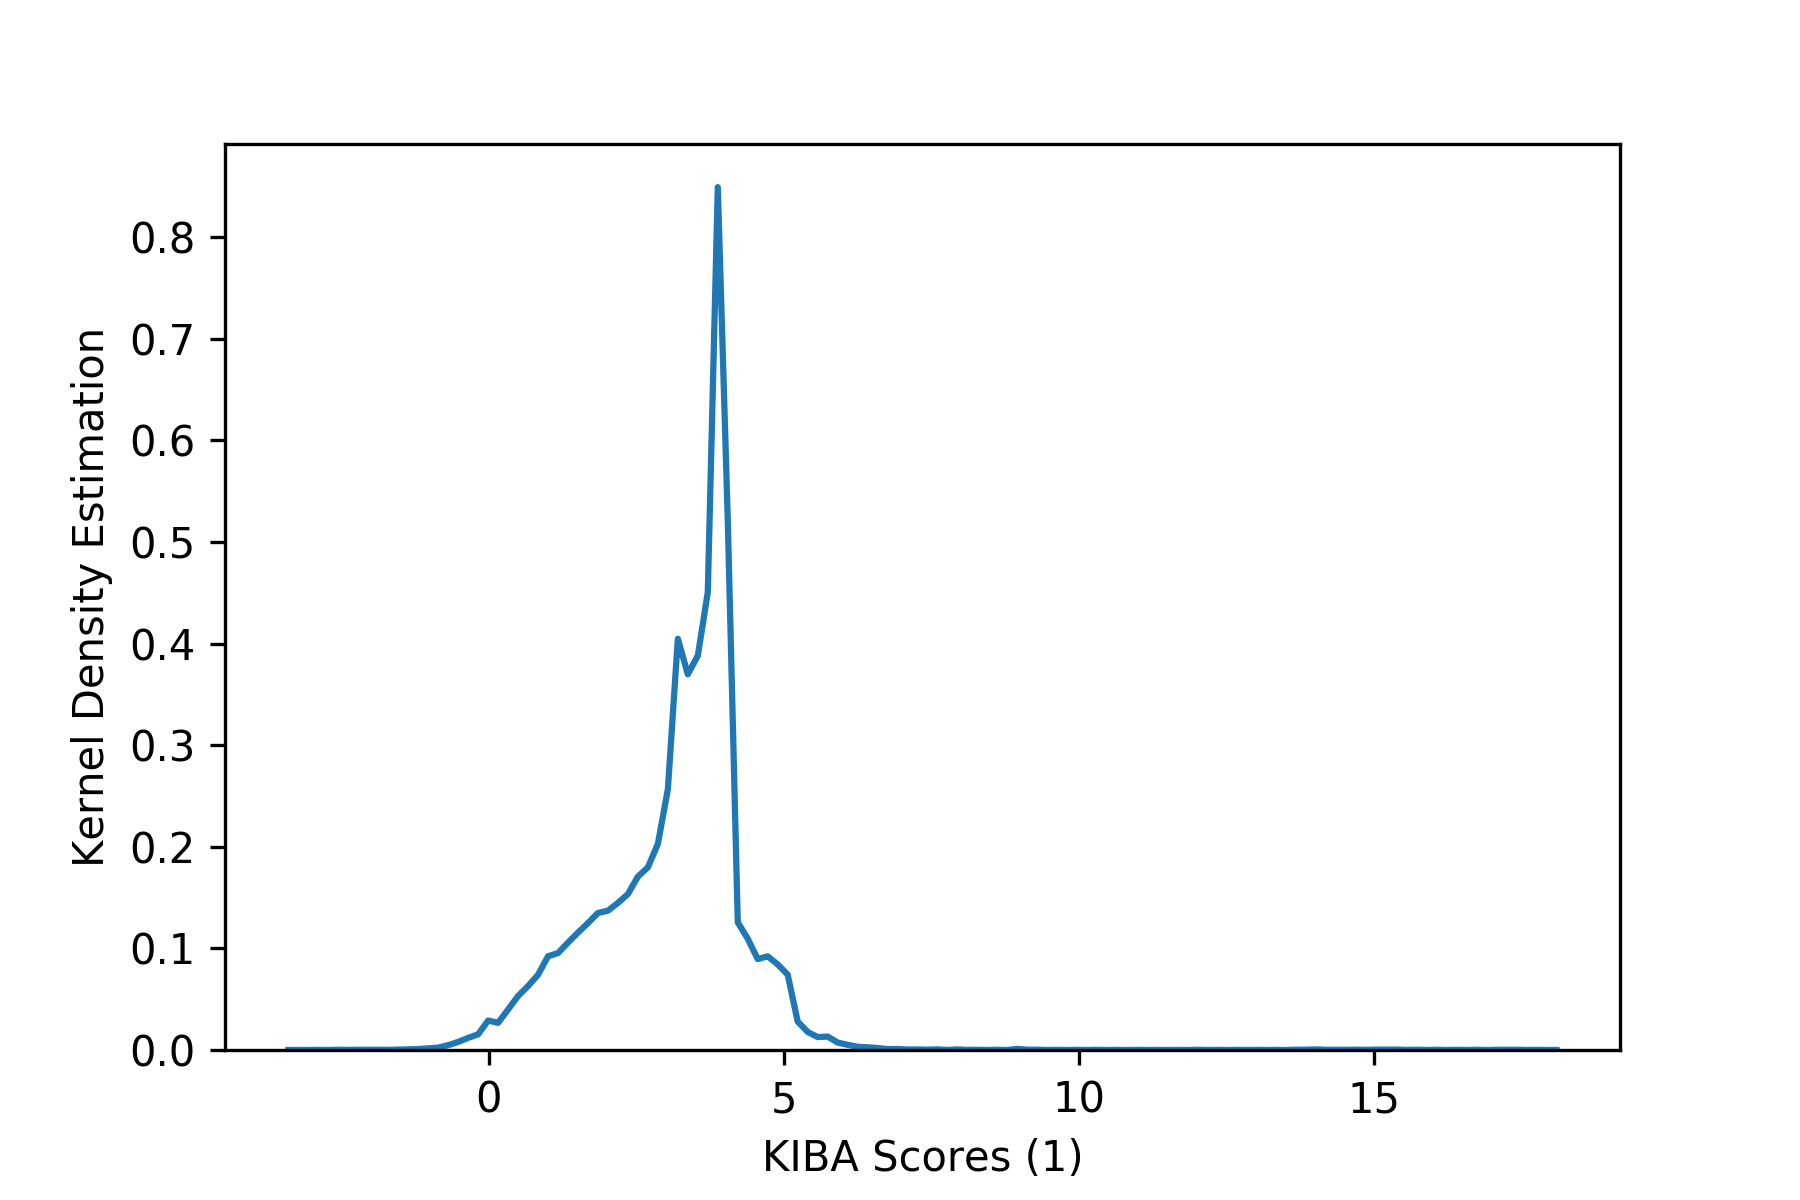
\includegraphics[width=.3\textwidth]{dataset/images/KIBA_scores.png}}
          
           \subfloat[][Drug-Protein Interaction]{
             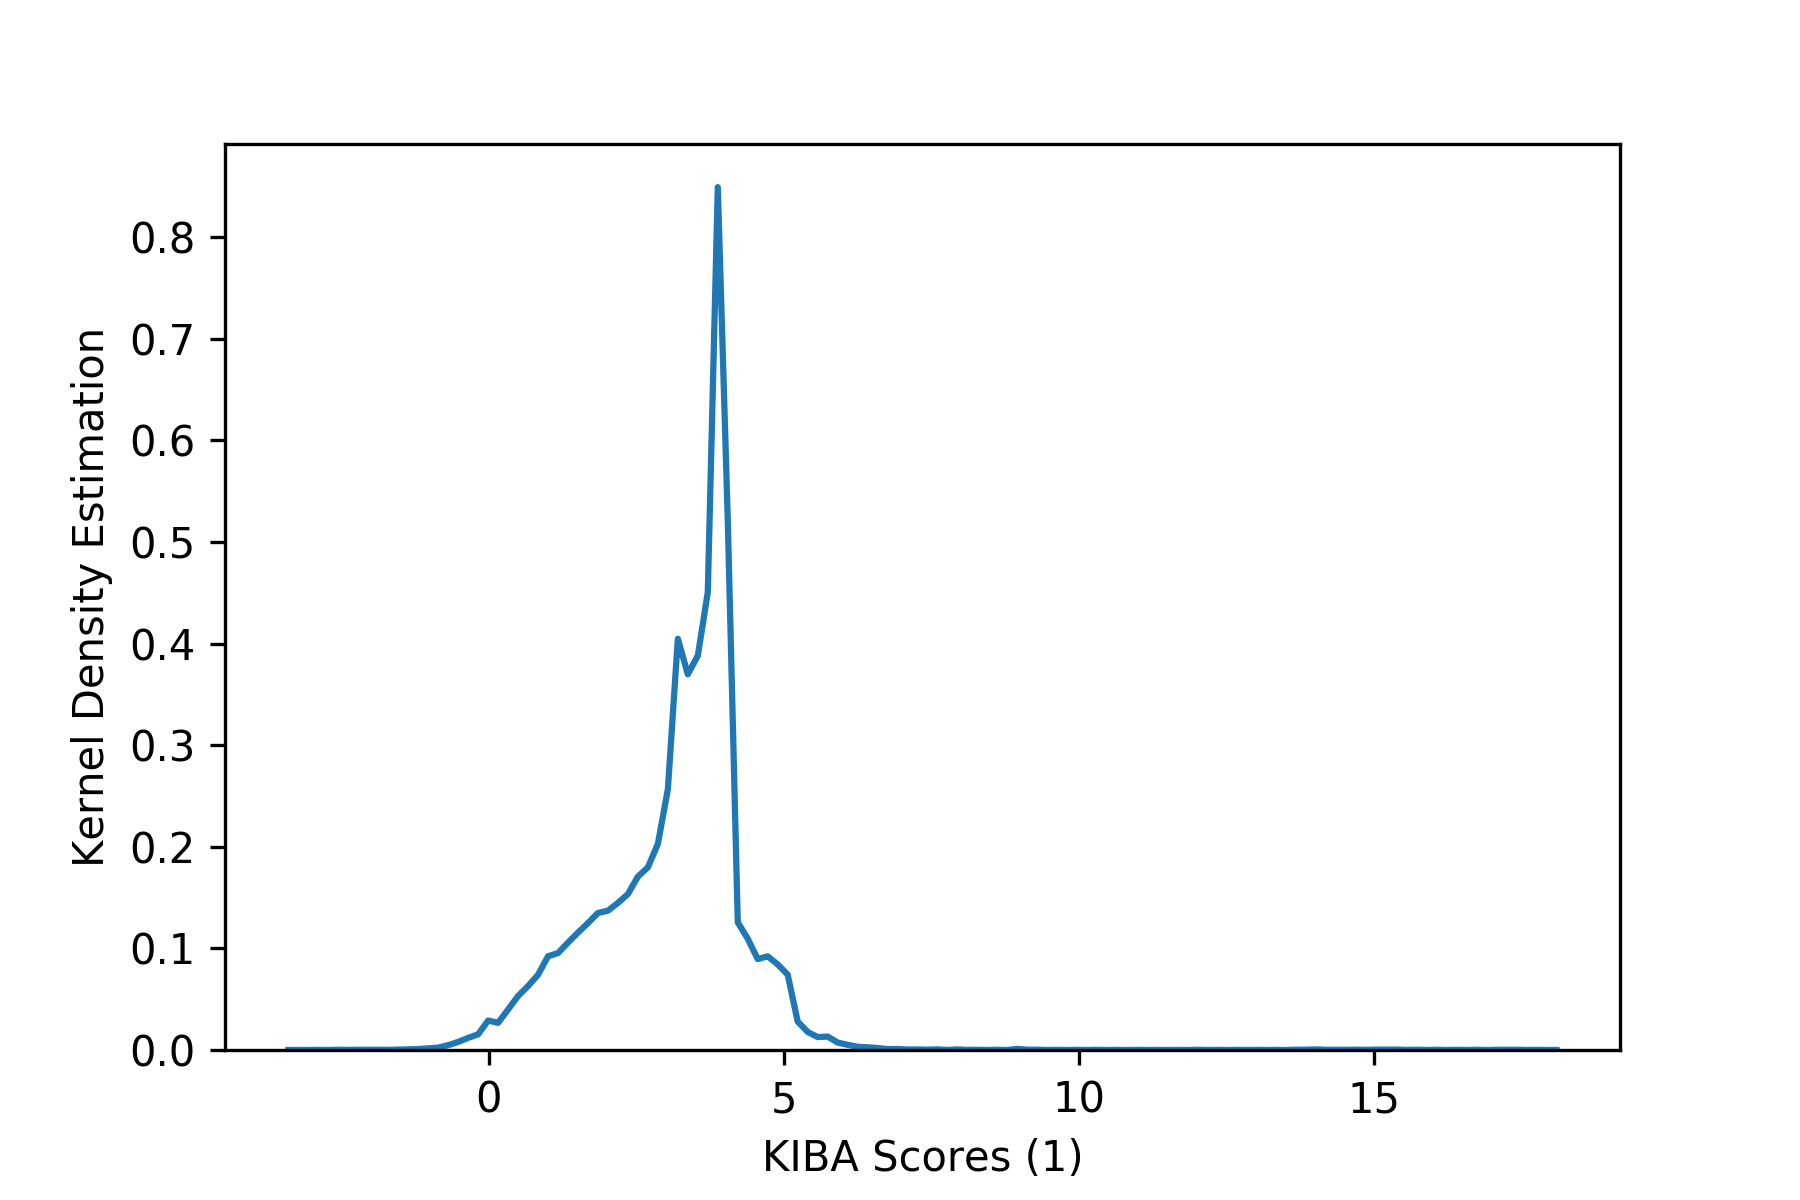
\includegraphics[width=.5\textwidth]{dataset/images/KIBA_scores.png}
             \label{fig:kiba_scores}
             }

           \subfloat[][Drugs SMILES Sequence]{
            \label{fig:drug_dist}  
            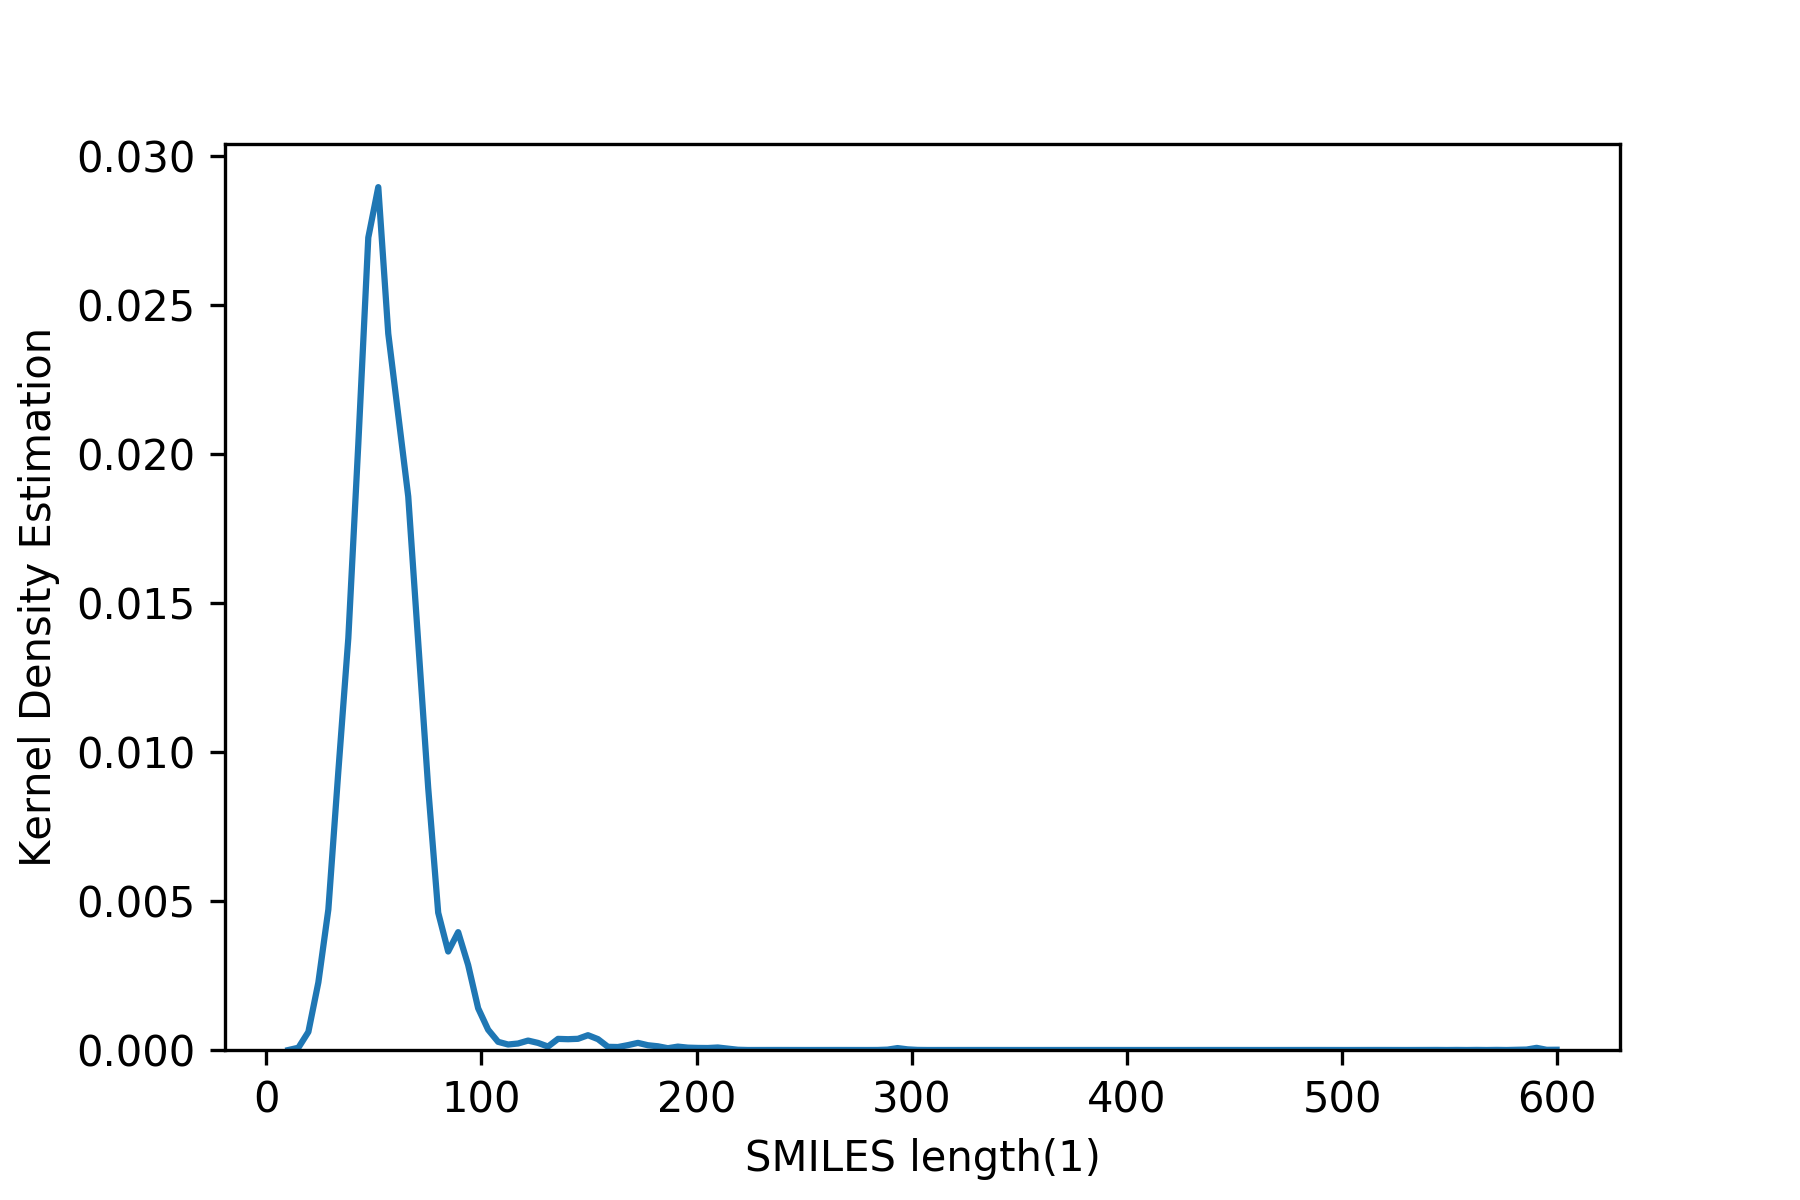
\includegraphics[width=.5\textwidth]{dataset/images/SMILES_distribution.png}
            }

           \subfloat[][Protein FASTA Sequence]{
             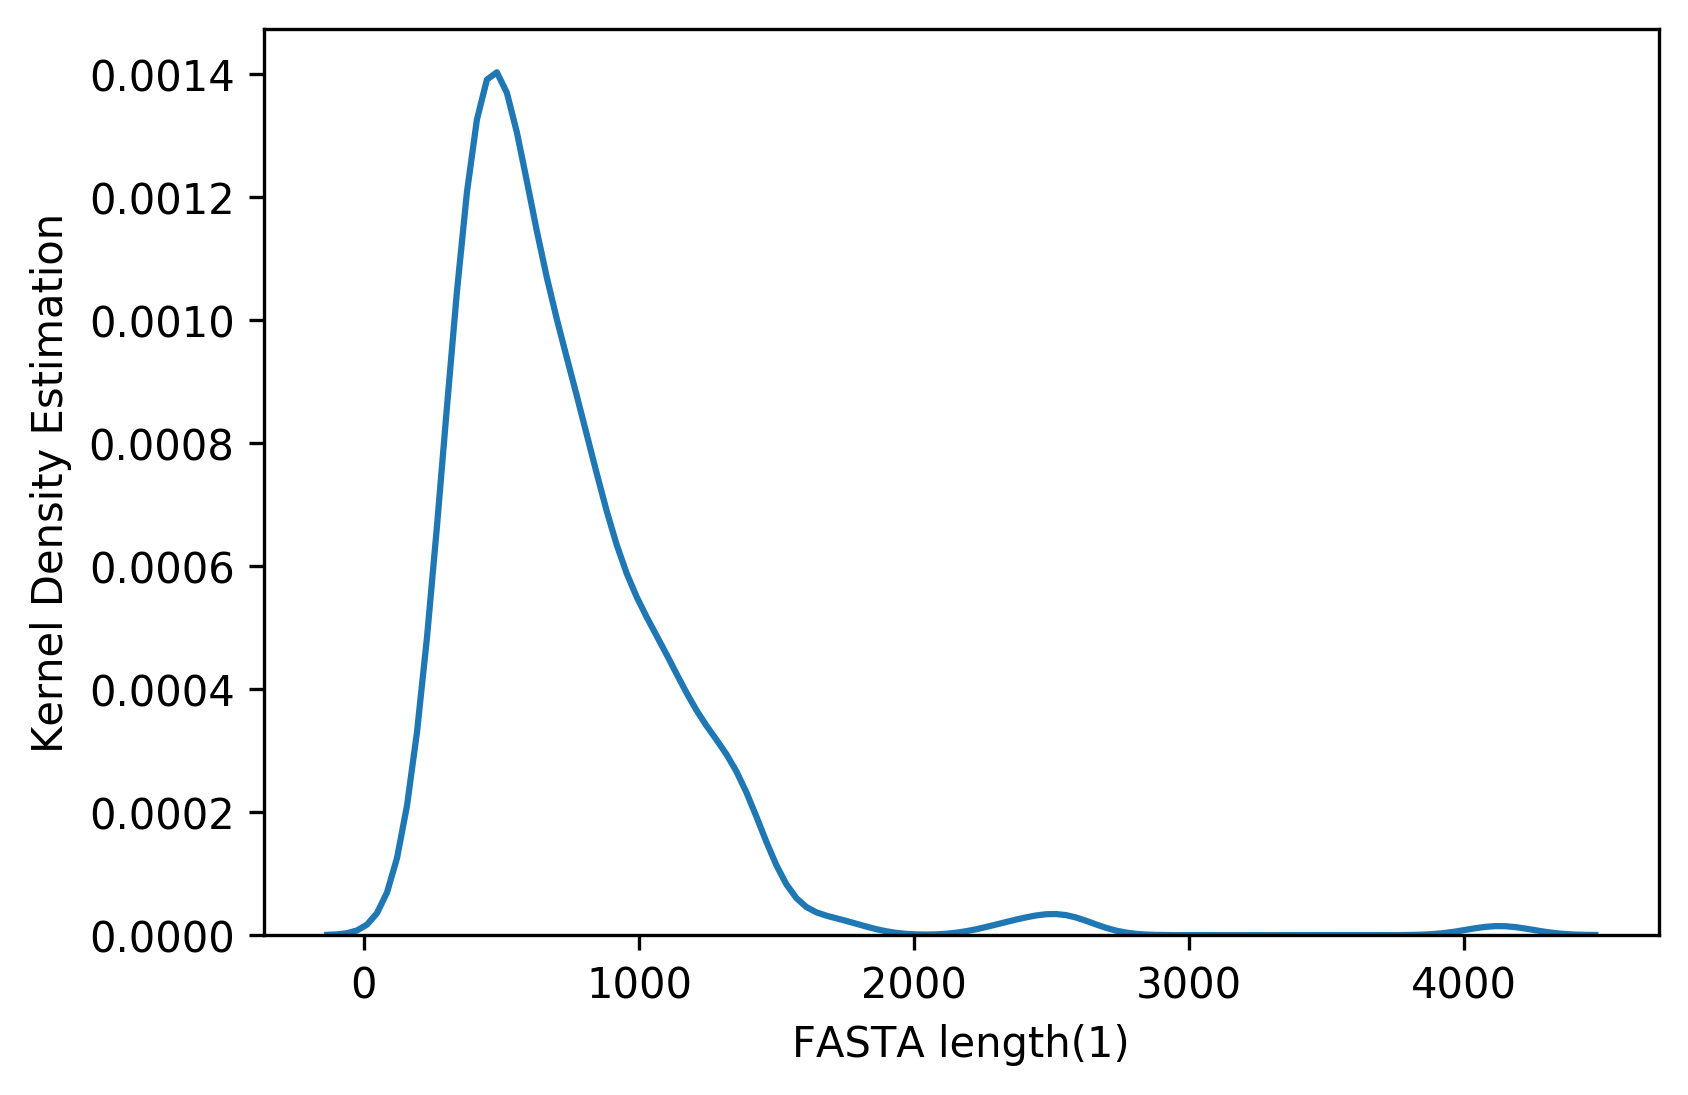
\includegraphics[width=.5\textwidth]{dataset/images/FASTA_distribution.png}
             \label{fig:prot_dist}
            }

           \caption[KDE Distribution]{Kernel Density Estimation Distribution of KIBA-interaction scores of Drug Sequences and Protein Sequences. \ref{sub@fig:kiba_scores} Distribution of KIBA Scores in Protein-Drug Interaction Pair, \ref{sub@fig:drug_dist} Distribution of length in Labeled Encodings of Drug Sequence, \ref{sub@fig:prot_dist} Distribution of length in Labelled Encodings Protein Sequence }
           \label{fig:kiba_drug_protein}
\end{figure}
  
\iffalse
  \subsection{UniProt and CHEMBL}
  
  \subsubsection{UniProt} 
  The sequence related information of protein is referenced using UniProt Identifier and protein sequence (FASTA) is called using the api from UniProt. \cite{UniProtConsortium2018}
  
  
  \subsubsection{CHEMBL}
  The molecular fingerprints related to drugs are referenced usning CHEMBL Identifier and the drug sequence is called from CHEMBL database. \cite{Gaulton2017}
  \fi
  \subsection{PSI-BLAST}
  PSI-Blast tools relates with multiple sequence alignments from a family of protein sequences\cite{Schaffer2001}. This helps to create a \acrshort{pssm} - Equation (\ref{eq:pssm}) - matrix referred to as secondary protein structure. For this study, the PSSM profile of every protein sequence is obtained by executing iteration of PSI-BLAST against \cite[KEGG]{Schaffer2001} protein. PSSM profile is a matrix of L*20 dimensions whereby 20 is the standard type of amino acids and L being the length of the protein. The larger positive scores represent conserved positions, which in turn implies critical functional residues that are required to perform various intermolecular interactions.\cite[PSSM]{Schaffer2001}
  
  \begin{equation}
    PSSM = \begin{bmatrix}
      P_{1,1} & P_{1,2} & \dots & P_{1,20} \\
      P_{2,1} & P_{2,2} & \dots & P_{2,20} \\
      \vdots  & \vdots  & \ddots & \vdots \\
      P_{L,1} & P_{L,2} & \dots & P_{L,20} \\
    \end{bmatrix}
    \label{eq:pssm}
  \end{equation}
  
  \subsubsection{PSSM-DT}
  Two forms of \acrshort{pssm} distance transformation techniques are used to transform the \acrshort{pssm} information into fixed dimensional vectors \cite{Xu2015}. The PSSM-DT (PSSM-Distance Transformation) can transform the \acrshort{pssm} information into uniform numeric representation by approximately measuring the occurrence probabilities of any pairs of amino acid. It results in two types of feature matrices: PSSM-SDT and PSSM-DDT defined by:
  
  \begin{equation}[H]
    PSSM-SDT(i,lg) = \sum_{i=1}^{L-lg} S_{i,j} \times \frac{ S_{i,j+lg} }{L-lg} 
    \label{eq:pssmsdt}
  \end{equation}
  \textit{\center lg =  distance of separation between same amino acid sequence}
  
  \begin{equation}[H]
    PSSM-DDT(i_1,i_2, lg) = \sum_{j=1}^{L-lg} S_{i_1,j} \times \frac{ S_{i_2,j+lg} }{ L-lg} 
    \label{eq:pssmddt}
  \end{equation}
  \textit{\centering i\textsubscript{1} and i\textsubscript{2} refer to tow different types of amino acids}
  
  Thus we have [380 ~\eqref{eq:pssmddt}+20 ~\eqref{eq:pssmsdt} = 400] x lg matrix which will be used as protein-specific vector in this work.
  
  \subsubsection{Evolutionary Distance Transformation Matrix}
  The mutational information of protein can be more informative than the sequence information itself\cite{Zhang2014}. Evolutionary difference formula (EDF) is used to represent mutation difference between adjacent residues. Secondly, the PSSM is converted into 20 x 20 matrix (ED-PSSM). These extracts are the non co-occurrence probability for two amino acids separated by a certain distance \textit{d} in the protein from the PSSM profile. For example, d=1 implies that the two amino acids are consecutive; d=2 implies that there is one amino acid between the two. Next, the EDT feature vector computed from ED-PSSM can be represented as (~\ref{eq:Pmat}): 
  \begin{equation}
    \label{eq:Pmat}
    P = [ \partial_1 ,\partial_2, \dots, \partial_\Omega]
  \end{equation}
  where $\Omega$ is an integer that represents the dimension of the vector whose value is 400.. The non-co-occurrence probability of two amino acids separated by distance \textit{d} can be computed as:
  \begin{equation}
    f(A_x,A_y) = \sum_{d=1}^{D} \frac{1}{L-d} \sum_{i=1}^{L-d} (P_{i,x} - P_{i+d,y})^2
    \label{eq:edt}
  \end{equation}
  where $P_{i,x}$ and $P_{i+d,y}$ are the elements in the PSSM profile; $A_x$ and $A_y$ represent any of the the 20 different amino acids in the protein sequence. Finally we spread the $f(A_x,A_y)$ in equation ~\ref{eq:Pmat} as:
  $ \partial_1 = f(A_1,A_2) $, 
  $ \partial_{400} = f(A_{20}, A_{20}) $
  
  
  \subsection{Residue feature} 
  The Statistical Residue Vector Space \acrshort{srv} \cite{Wong2018} plays an important role in Residue Residue Interaction and creates a basis for structural stability of the protein sequence itself. It is related to the tertiary structure of the protein sequence. Nonetheless, another function is to create a correlated sequence of information whereby two proteins are distantly related by sequence. Simultaneously, it is highly related to the functional characteristic of protein.  With this, table ~\ref{table:r2r} as attached in Appendix depicts a 20 x 20 matrix whose rows and columns represent 20 standard amino acids.
  
  \subsubsection{Residue Probing Transformation(RPT) feature}
  RPT as proposed by Jeong et al.\cite{Jeong2011}, and implemented by Pujan et al.\cite{Mishra2019}, emphasize domains with similar conservation rates by grouping domain families based on their conservation score in the PSSM profile.
  \begin{equation}
    RPT = \begin{bmatrix}
      S_{1,1} & S_{1,2} & \dots & S_{1,20} \\
      S_{2,1} & S_{2,2} & \dots & S_{2,20} \\
      \vdots  & \vdots  & \ddots & \vdots \\
      S_{2,1} & S_{2,2} & \dots & S_{2,20} \\
    \end{bmatrix}
    \label{eq:rpt}
  \end{equation}
  The RPT matrix (Equation ~\ref{eq:rpt}) is then tranformed into feature vector of 400 dimensions, as shown in Equation ~\ref{eq:rptV}.
  
  \begin{equation}
    V = [ f_{s_{1,1}}, f_{s_{1,2}}, \dots, f_{s_{i,j}}, \dots, f_{s_{20,20}} ]
    \label{eq:rptV}
  \end{equation}
  where, 
  \begin{equation}
    f_{s_{i,j}} = \frac{s_{i,j}}{L} (i,j = 1,2,\dots,20)
    \label{eq:rptF}
  \end{equation}

  \subsection{Labelled Encodings}
  
  The labeled encoding techniques is used to represent the canonical structure of drugs and proteins. The structural canonical information is preserved while sending the feature set to deep learning method. An array of integers are formed from particular sequence while representing the structural information.
  
  The Labelled Encodings of protein and drugs can be defined by table \ref{table:label_encoding} :
  \begin{table}[H]
    \centering
    \caption{Labeled Encoding of Proteins and Drugs}
    \label{table:label_encoding}
    \qquad
    \subfloat[][Label Encodings for Proteins]{
      \label{table:label_encoding:prot}
      \begin{tabular}{|cccc|}
        \hline
        A --> 1 & C --> 2 & B --> 3 & E --> 4 \\ \hline
        D --> 5 & G --> 6 & F --> 7 & I --> 8 \\ \hline
      \end{tabular}
      }

    \qquad
    \subfloat[][Label Encodings for Drugs]{
      \label{table:label_encoding:drugs}
      \centering
      % \caption{Drugs Labeled Encoding Technique}
      \begin{tabular}{|cccc|}
        \hline
        \# --> 1 & \% --> 2 & : --> 3 & + --> 5 \\ \hline
        4 --> 13 & 7 --> 14 & F --> 25 & I --> 26 \\ \hline
      \end{tabular}
      }
  \end{table}
  
  % CHARPROTSET = { "A": 1, "C": 2, "B": 3, "E": 4, "D": 5, "G": 6,
	% 			"F": 7, "I": 8, "H": 9, "K": 10, "M": 11, "L": 12,
	% 			"O": 13, "N": 14, "Q": 15, "P": 16, "S": 17, "R": 18,
	% 			"U": 19, "T": 20, "W": 21,
	% 			"V": 22, "Y": 23, "X": 24,
	% 			"Z": 25 }

  % CHARCANSMISET = { "#": 1, "%": 2, ")": 3, "(": 4, "+": 5, "-": 6,
	% 		 ".": 7, "1": 8, "0": 9, "3": 10, "2": 11, "5": 12,
	% 		 "4": 13, "7": 14, "6": 15, "9": 16, "8": 17, "=": 18,
	% 		 "A": 19, "C": 20, "B": 21, "E": 22, "D": 23, "G": 24,
	% 		 "F": 25, "I": 26, "H": 27, "K": 28, "M": 29, "L": 30,
	% 		 "O": 31, "N": 32, "P": 33, "S": 34, "R": 35, "U": 36,
	% 		 "T": 37, "W": 38, "V": 39, "Y": 40, "[": 41, "Z": 42,
	% 		 "]": 43, "_": 44, "a": 45, "c": 46, "b": 47, "e": 48,
	% 		 "d": 49, "g": 50, "f": 51, "i": 52, "h": 53, "m": 54,
	% 		 "l": 55, "o": 56, "n": 57, "s": 58, "r": 59, "u": 60,
	% 		 "t": 61, "y": 62 }
  
  \subsection{Position Specific Score Matrix}

\acrfull{pssm} is a very useful protein feature. The protein feature represented by PSSM depends on the sequence of all the proteins in consideration. The HUMAN genome protein (a database of more than 100,000) is downloaded from UniProt Library. The PSSM matrix is constructed for each of the kinase proteins based on this HUMAN Genome Protein Database. With this, the PSSM matrix is characterized according to human proteins to anticipate the prediction of new identified kinase proteins.

\begin{table}
  \centering
  {\caption{PSSM Analysis Design}
  \label{table:PSSM_Analysis} }
    \subfloat[][Protein FASTA Sequence]{
      \label{table:PSSM_Analysis:fasta} 
      \begin{tabular}{|l|l|} \toprule
      \hline
      1 & GAGGTAAAC \\ \hline
      2 & TCCGTAAGT \\ \hline
      3 & CAGGTTGGA \\ \hline
      4 & ACAGTCAGT \\ \hline
      5 & TAGGTCATT \\ \hline
      6 & TAGGTACTG \\ \hline
      7 & ATGGTAACT \\ \hline
      8 & CAGGTATAC \\ \hline
      9 & TGTGTGAGT \\ \hline
      10 & AAGGTAAGT \\ \hline
      
      \end{tabular}
    }
    \subfloat[][Frequency Table]{
      \label{table:PSSM_Analysis:frequency}
      \begin{tabular}{|l|l|l|l|l|l|l|l|l|l|} \toprule
        \hline
        
         & 1 & 2 & 3 & 4 & 5 & 6 & 7 & 8 & 9 \\ \hline
        A & 3 & 6 & 1 & 0 & 0 & 6 & 7 & 2 & 1 \\ \hline
        C & 2 & 2 & 1 & 0 & 0 & 2 & 1 & 1 & 2 \\ \hline
        G & 1 & 1 & 7 & 10 & 0 & 1 & 1 & 5 & 1 \\ \hline
        T & 4 & 1 & 1 & 0 & 10 & 1 & 1 & 2 & 6 \\ \hline
        
        \end{tabular}

    } 
  
  
  \subfloat[][Log-Likelihood Matrix]{
    % \rule{4cm}{0cm}
    \begin{tabular}{|l|l|l|l|l|l|l|l|l|l|} \toprule
      \hline 
  
          & 1 & 2 & 3 & 4 & 5 & 6 & 7 & 8 & 9 \\ \hline
      A & 0.3 & 0.6 & 0.1 & 0.00 & 0.00 & 0.6 & 0.7 & 0.2 & 0.1 \\ \hline
      C & 0.2 & 0.2 & 0.1 & 0.00 & 0.00 & 0.2 & 0.1 & 0.1 & 0.2 \\ \hline
      G & 0.1 & 0.1 & 0.7 & 1.00 & 0.00 & 0.1 & 0.1 & 0.5 & 0.1 \\ \hline
      T & 0.4 & 0.1 & 0.1 & 0.00 & 1.00 & 0.1 & 0.1 & 0.2 & 0.6 \\ \hline
      
      \end{tabular}  
      \label{table:log_likelihood_pssm}
    }
    
  
  \subfloat[][Sliding Window Score Calculation]{
    \centering
    \begin{tabular}{|l|l|l|l|l|l|l|l|l|l|}
    \hline 
    
        & 1 & 2 & 3 & 4 & 5 & 6 & 7 & 8 & 9 \\ \hline
    A & 0.3 &  &  &  &  &  & 0.7 &  &  \\ \hline
    C &  &  & 0.1 & 0.00 & 0.00 & 0.20 &  &  & 0.2 \\ \hline
    G &  & 0.1 &  &  &  &  &  & 0.5 &  \\ \hline
    T &  &  &  &  &  &  &  &  &  \\ \hline
    
    \end{tabular}  
    \label{table:motif_movement}
    }

    
    \subfloat[][Score of sliding window motifs]{
    \label{wrapTable:pssm-score}
    \begin{tabular}{|l|l|l|l|l|l|l|l|l|l|}
      \hline
      0 & 1 & 2 & 3 & 4 & 5 & 6 & 7 & 8 & 9 \\ \hline
      1.099 & 1 & 2.2 & 2.1 & 2.1 & 1.300 & 1.3 & 1.4 & 2 & 2.9 \\ \hline
      \end{tabular}
    }
\end{table}

Table \ref{table:PSSM_Analysis} shows a conventional process of calculating PSSM score values. The sequence following shows the process of calculating the scores once the PSSM distribution of the whole family is calculated. Table \ref{table:motif_movement} shows the score distribution of lowercase amino acid sequence (starting after 4th position) determined by the size of the sliding window.

\seqsplit{ACTC\textbf{agccccagc}GGAGGTGAAGGACGTCCTTCCCCAGGAGCCGGTGAGAAGCGCAGTCGGGGGCACGGGGATGAGCTCAGGGGCCTCTAGAAAGATGTAGCTGGGACCTCGGGAAGCCCTGGCCTCCAGGTAGTCTCAGGAGAGCTACTCAGGGTCGGGCTTGGGGAGAGGAGGAGCGGGGGTGAGGCCAGCAGCA} 

% % \begin{wraptable}{br}{5.5cm}
% \begin{table}[H]
%     \centering
    
% \end{table}
% % \end{wraptable}

.3, .1, .1, 0, 0, .2, .7, .5, .2  == Sum(2.1) - posix(4) -- See table \ref{wrapTable:pssm-score}

\begin{figure}[htbp]
    \centering 
          %  \subfloat[]{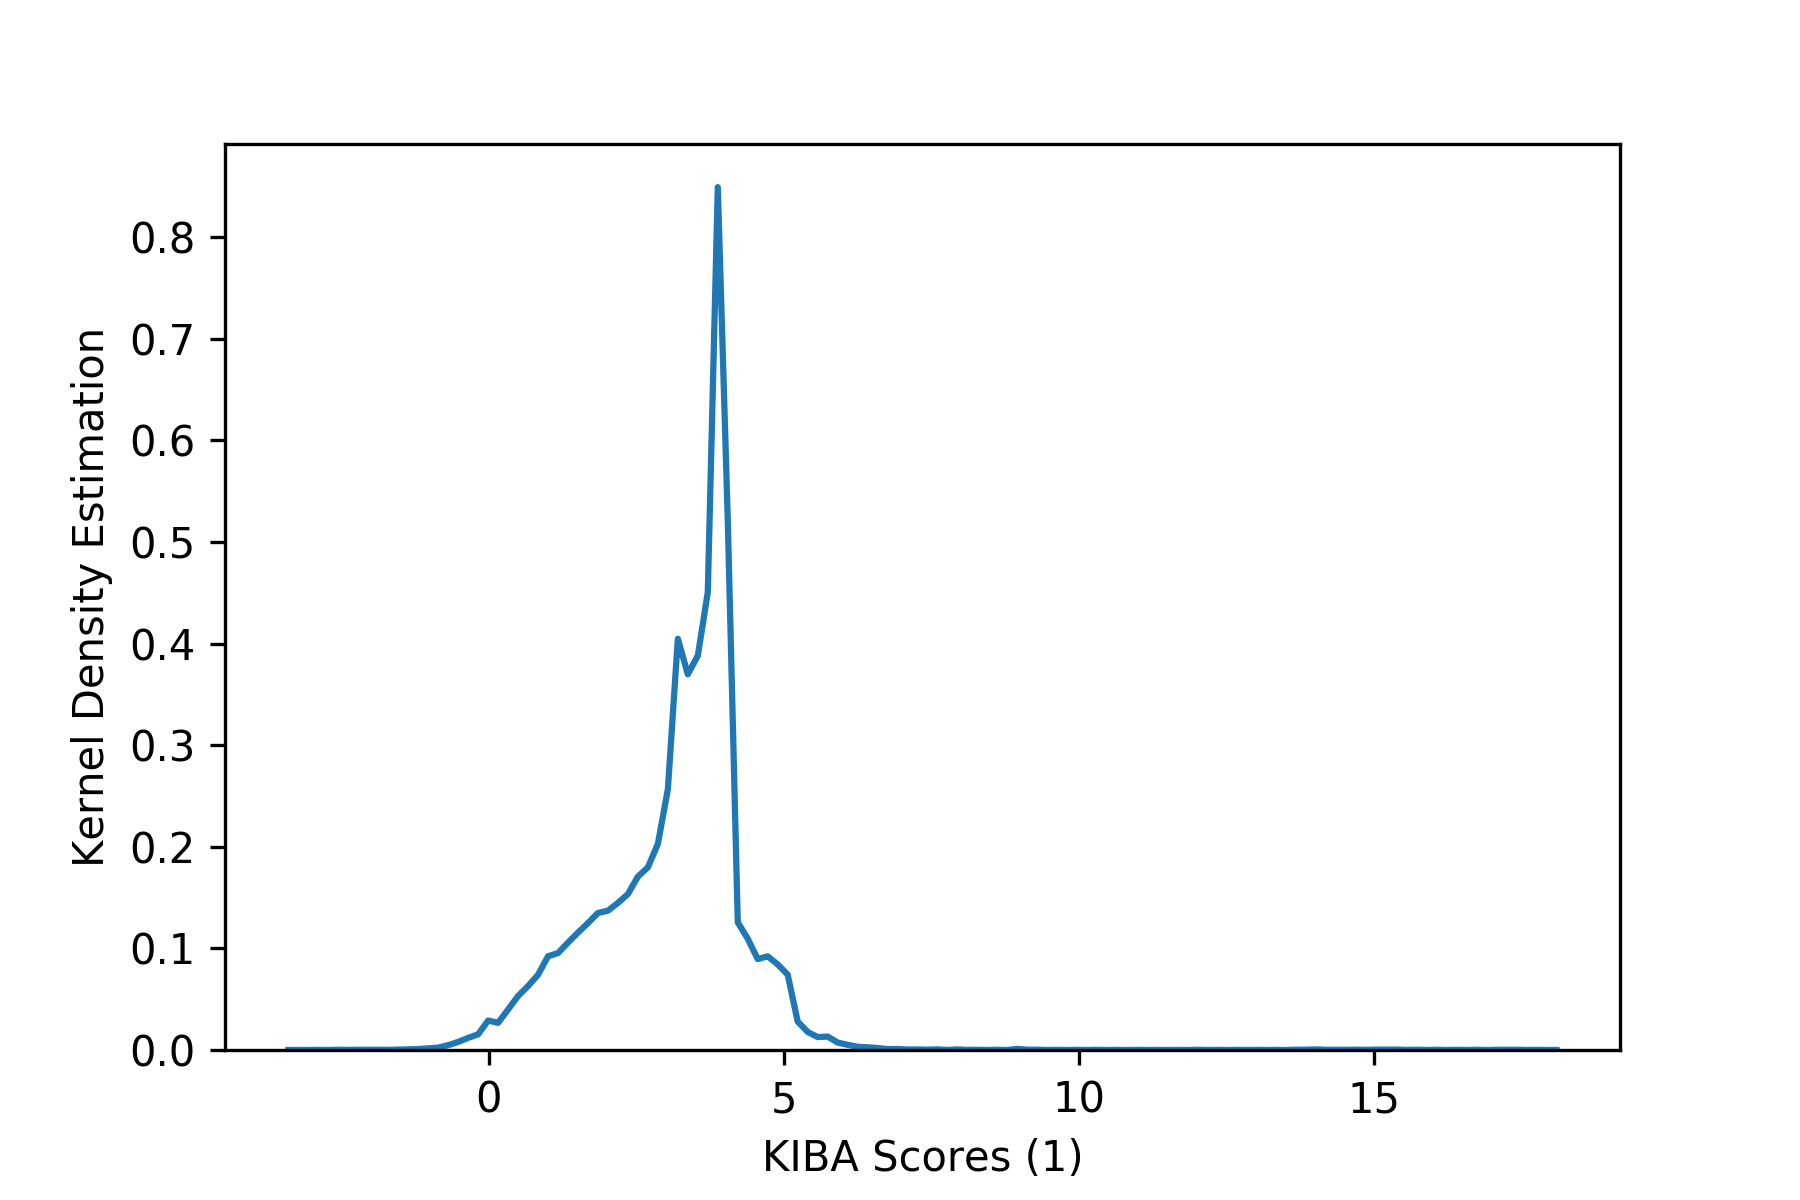
\includegraphics[width=.3\textwidth]{dataset/images/KIBA_scores.png}}
          
           \subfloat[][Drug-Protein Interaction]{
             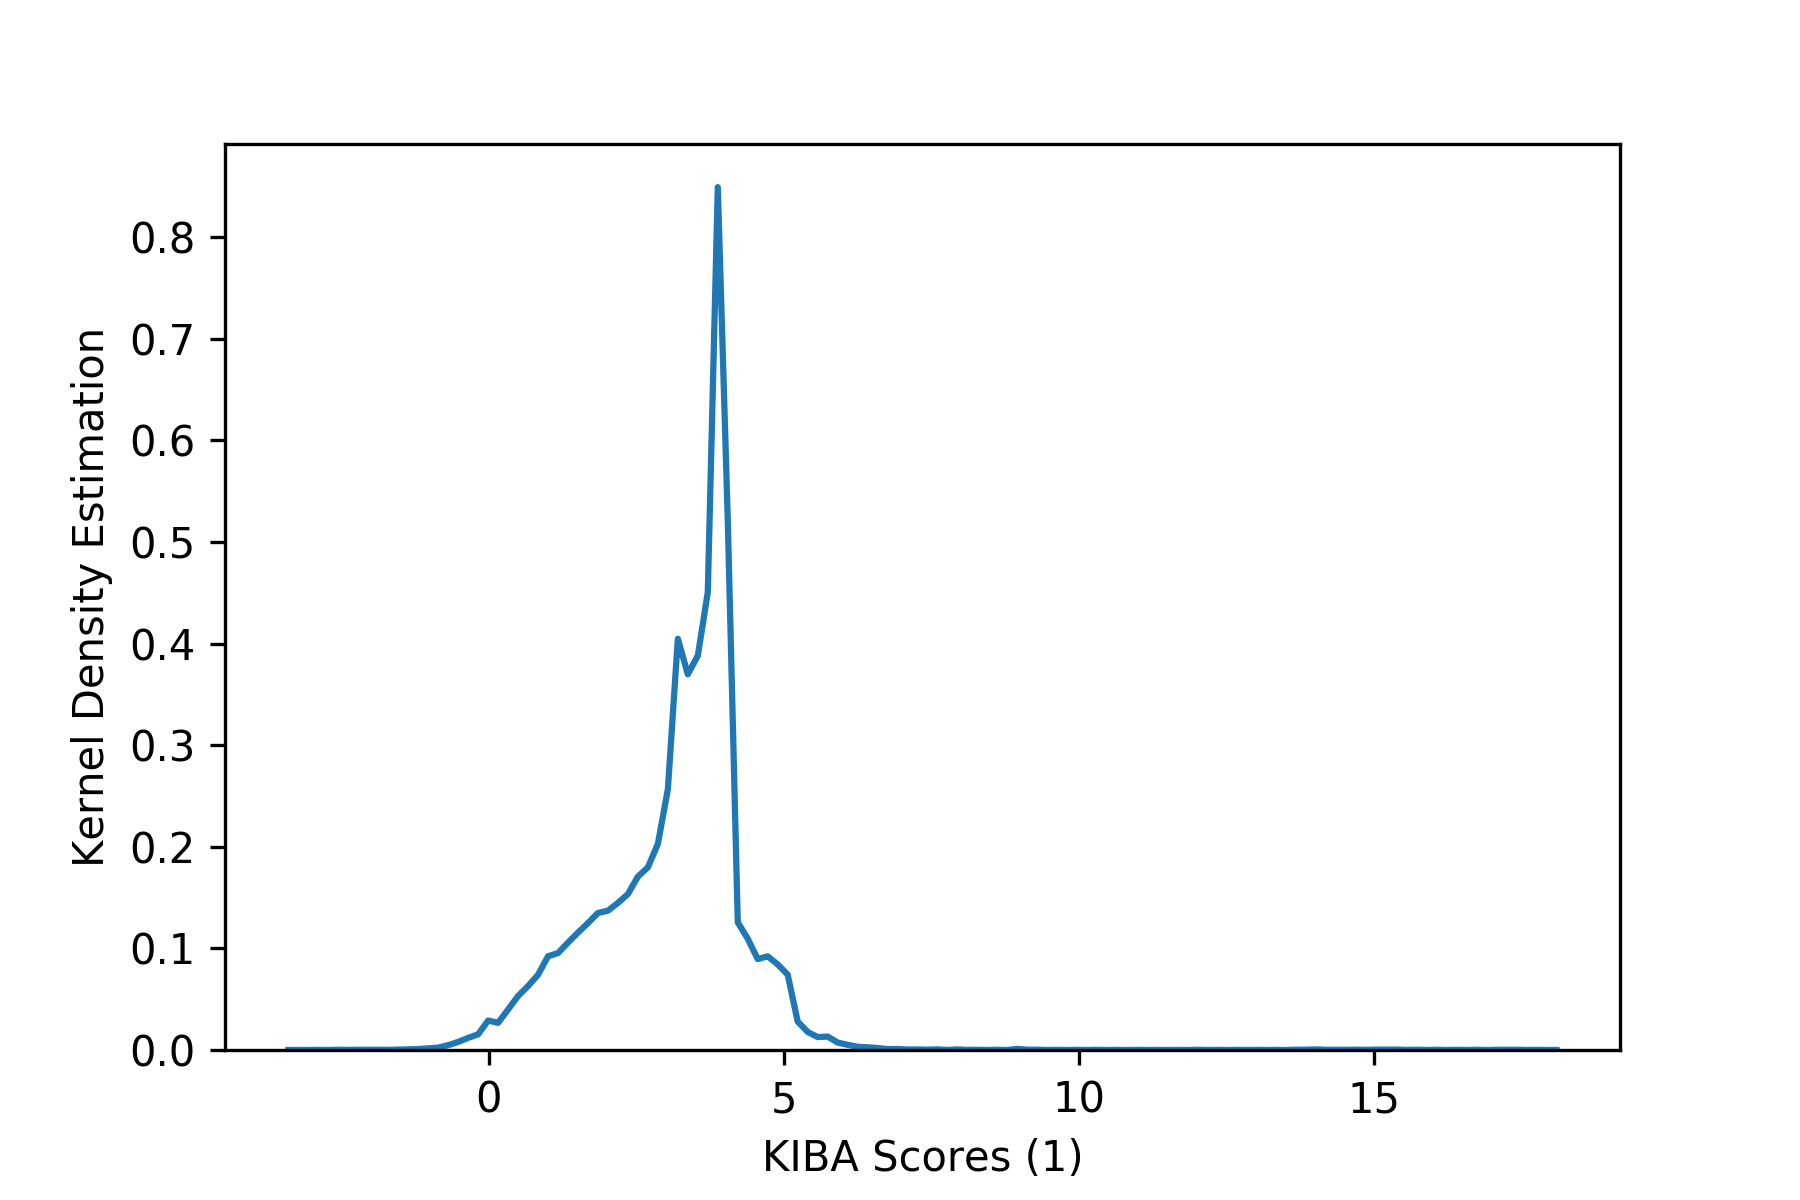
\includegraphics[width=.5\textwidth]{dataset/images/KIBA_scores.png}
             \label{fig:kiba_scores}
             }

           \subfloat[][Drugs SMILES Sequence]{
            \label{fig:drug_dist}  
            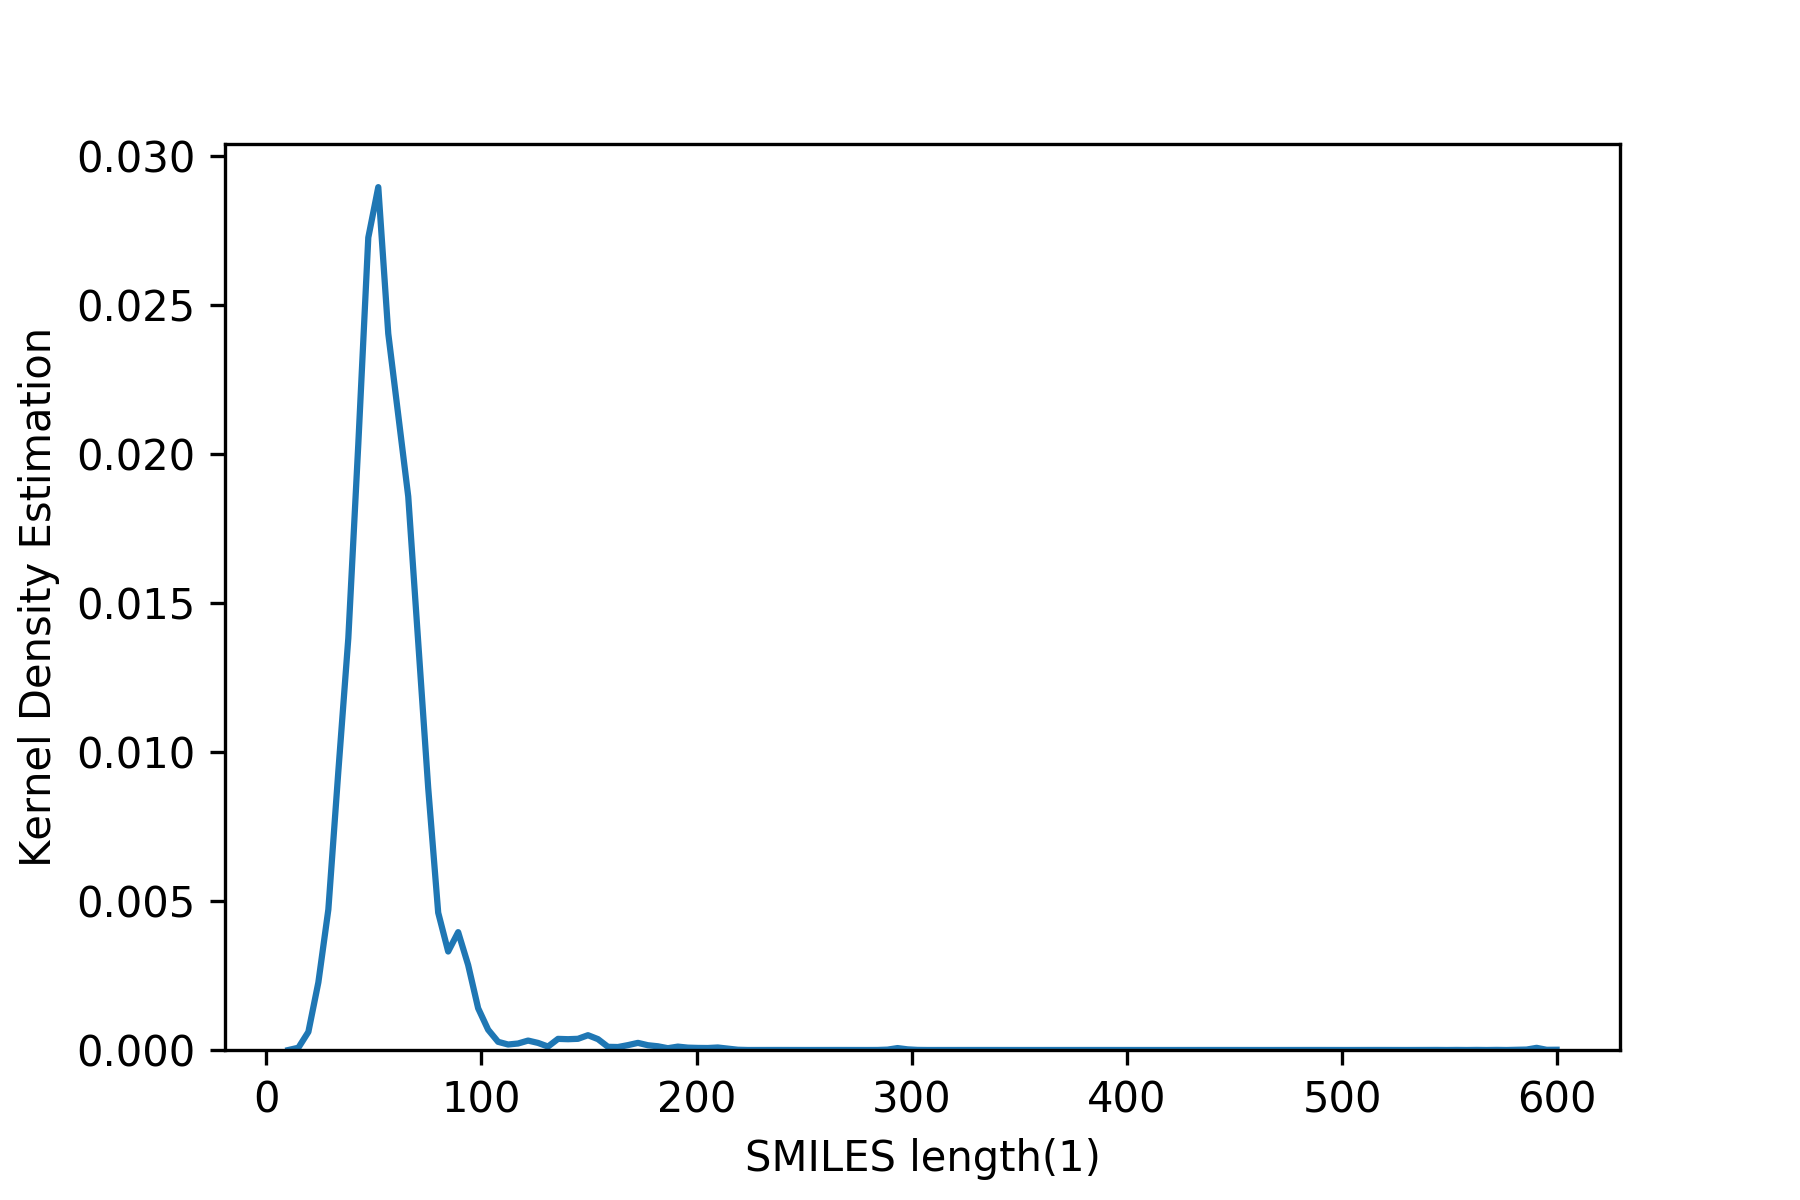
\includegraphics[width=.5\textwidth]{dataset/images/SMILES_distribution.png}
            }

           \subfloat[][Protein FASTA Sequence]{
             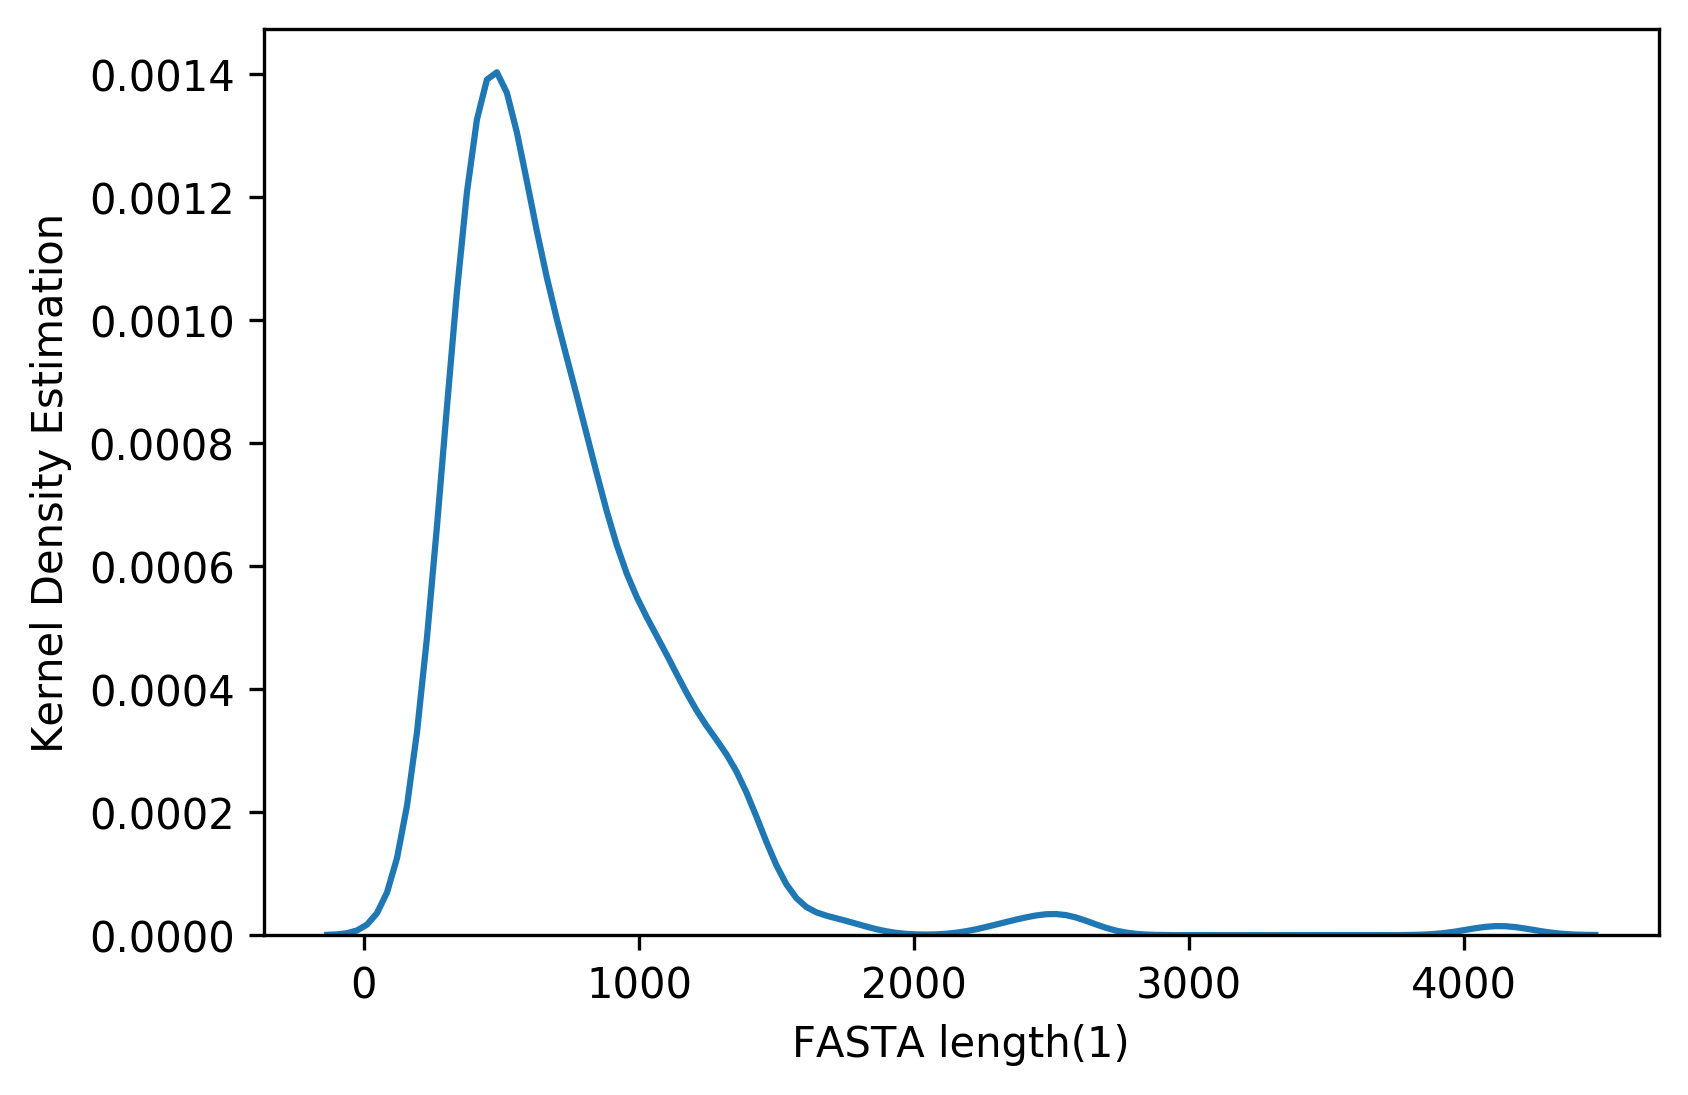
\includegraphics[width=.5\textwidth]{dataset/images/FASTA_distribution.png}
             \label{fig:prot_dist}
            }

           \caption[KDE Distribution]{Kernel Density Estimation Distribution of KIBA-interaction scores of Drug Sequences and Protein Sequences. \ref{sub@fig:kiba_scores} Distribution of KIBA Scores in Protein-Drug Interaction Pair, \ref{sub@fig:drug_dist} Distribution of length in Labeled Encodings of Drug Sequence, \ref{sub@fig:prot_dist} Distribution of length in Labelled Encodings Protein Sequence }
           \label{fig:kiba_drug_protein}
\end{figure}
  
\iffalse
  \subsection{UniProt and CHEMBL}
  
  \subsubsection{UniProt} 
  The sequence related information of protein is referenced using UniProt Identifier and protein sequence (FASTA) is called using the api from UniProt. \cite{UniProtConsortium2018}
  
  
  \subsubsection{CHEMBL}
  The molecular fingerprints related to drugs are referenced usning CHEMBL Identifier and the drug sequence is called from CHEMBL database. \cite{Gaulton2017}
  \fi
  \subsection{PSI-BLAST}
  PSI-Blast tools relates with multiple sequence alignments from a family of protein sequences\cite{Schaffer2001}. This helps to create a \acrshort{pssm} - Equation (\ref{eq:pssm}) - matrix referred to as secondary protein structure. For this study, the PSSM profile of every protein sequence is obtained by executing iteration of PSI-BLAST against \cite[KEGG]{Schaffer2001} protein. PSSM profile is a matrix of L*20 dimensions whereby 20 is the standard type of amino acids and L being the length of the protein. The larger positive scores represent conserved positions, which in turn implies critical functional residues that are required to perform various intermolecular interactions.\cite[PSSM]{Schaffer2001}
  
  \begin{equation}
    PSSM = \begin{bmatrix}
      P_{1,1} & P_{1,2} & \dots & P_{1,20} \\
      P_{2,1} & P_{2,2} & \dots & P_{2,20} \\
      \vdots  & \vdots  & \ddots & \vdots \\
      P_{L,1} & P_{L,2} & \dots & P_{L,20} \\
    \end{bmatrix}
    \label{eq:pssm}
  \end{equation}
  
  \subsubsection{PSSM-DT}
  Two forms of \acrshort{pssm} distance transformation techniques are used to transform the \acrshort{pssm} information into fixed dimensional vectors \cite{Xu2015}. The PSSM-DT (PSSM-Distance Transformation) can transform the \acrshort{pssm} information into uniform numeric representation by approximately measuring the occurrence probabilities of any pairs of amino acid. It results in two types of feature matrices: PSSM-SDT and PSSM-DDT defined by:
  
  \begin{equation}[H]
    PSSM-SDT(i,lg) = \sum_{i=1}^{L-lg} S_{i,j} \times \frac{ S_{i,j+lg} }{L-lg} 
    \label{eq:pssmsdt}
  \end{equation}
  \textit{\center lg =  distance of separation between same amino acid sequence}
  
  \begin{equation}[H]
    PSSM-DDT(i_1,i_2, lg) = \sum_{j=1}^{L-lg} S_{i_1,j} \times \frac{ S_{i_2,j+lg} }{ L-lg} 
    \label{eq:pssmddt}
  \end{equation}
  \textit{\centering i\textsubscript{1} and i\textsubscript{2} refer to tow different types of amino acids}
  
  Thus we have [380 ~\eqref{eq:pssmddt}+20 ~\eqref{eq:pssmsdt} = 400] x lg matrix which will be used as protein-specific vector in this work.
  
  \subsubsection{Evolutionary Distance Transformation Matrix}
  The mutational information of protein can be more informative than the sequence information itself\cite{Zhang2014}. Evolutionary difference formula (EDF) is used to represent mutation difference between adjacent residues. Secondly, the PSSM is converted into 20 x 20 matrix (ED-PSSM). These extracts are the non co-occurrence probability for two amino acids separated by a certain distance \textit{d} in the protein from the PSSM profile. For example, d=1 implies that the two amino acids are consecutive; d=2 implies that there is one amino acid between the two. Next, the EDT feature vector computed from ED-PSSM can be represented as (~\ref{eq:Pmat}): 
  \begin{equation}
    \label{eq:Pmat}
    P = [ \partial_1 ,\partial_2, \dots, \partial_\Omega]
  \end{equation}
  where $\Omega$ is an integer that represents the dimension of the vector whose value is 400.. The non-co-occurrence probability of two amino acids separated by distance \textit{d} can be computed as:
  \begin{equation}
    f(A_x,A_y) = \sum_{d=1}^{D} \frac{1}{L-d} \sum_{i=1}^{L-d} (P_{i,x} - P_{i+d,y})^2
    \label{eq:edt}
  \end{equation}
  where $P_{i,x}$ and $P_{i+d,y}$ are the elements in the PSSM profile; $A_x$ and $A_y$ represent any of the the 20 different amino acids in the protein sequence. Finally we spread the $f(A_x,A_y)$ in equation ~\ref{eq:Pmat} as:
  $ \partial_1 = f(A_1,A_2) $, 
  $ \partial_{400} = f(A_{20}, A_{20}) $
  
  
  \subsection{Residue feature} 
  The Statistical Residue Vector Space \acrshort{srv} \cite{Wong2018} plays an important role in Residue Residue Interaction and creates a basis for structural stability of the protein sequence itself. It is related to the tertiary structure of the protein sequence. Nonetheless, another function is to create a correlated sequence of information whereby two proteins are distantly related by sequence. Simultaneously, it is highly related to the functional characteristic of protein.  With this, table ~\ref{table:r2r} as attached in Appendix depicts a 20 x 20 matrix whose rows and columns represent 20 standard amino acids.
  
  \subsubsection{Residue Probing Transformation(RPT) feature}
  RPT as proposed by Jeong et al.\cite{Jeong2011}, and implemented by Pujan et al.\cite{Mishra2019}, emphasize domains with similar conservation rates by grouping domain families based on their conservation score in the PSSM profile.
  \begin{equation}
    RPT = \begin{bmatrix}
      S_{1,1} & S_{1,2} & \dots & S_{1,20} \\
      S_{2,1} & S_{2,2} & \dots & S_{2,20} \\
      \vdots  & \vdots  & \ddots & \vdots \\
      S_{2,1} & S_{2,2} & \dots & S_{2,20} \\
    \end{bmatrix}
    \label{eq:rpt}
  \end{equation}
  The RPT matrix (Equation ~\ref{eq:rpt}) is then tranformed into feature vector of 400 dimensions, as shown in Equation ~\ref{eq:rptV}.
  
  \begin{equation}
    V = [ f_{s_{1,1}}, f_{s_{1,2}}, \dots, f_{s_{i,j}}, \dots, f_{s_{20,20}} ]
    \label{eq:rptV}
  \end{equation}
  where, 
  \begin{equation}
    f_{s_{i,j}} = \frac{s_{i,j}}{L} (i,j = 1,2,\dots,20)
    \label{eq:rptF}
  \end{equation}

  \subsection{Labelled Encodings}
  
  The labeled encoding techniques is used to represent the canonical structure of drugs and proteins. The structural canonical information is preserved while sending the feature set to deep learning method. An array of integers are formed from particular sequence while representing the structural information.
  
  The Labelled Encodings of protein and drugs can be defined by table \ref{table:label_encoding} :
  \begin{table}[H]
    \centering
    \caption{Labeled Encoding of Proteins and Drugs}
    \label{table:label_encoding}
    \qquad
    \subfloat[][Label Encodings for Proteins]{
      \label{table:label_encoding:prot}
      \begin{tabular}{|cccc|}
        \hline
        A --> 1 & C --> 2 & B --> 3 & E --> 4 \\ \hline
        D --> 5 & G --> 6 & F --> 7 & I --> 8 \\ \hline
      \end{tabular}
      }

    \qquad
    \subfloat[][Label Encodings for Drugs]{
      \label{table:label_encoding:drugs}
      \centering
      % \caption{Drugs Labeled Encoding Technique}
      \begin{tabular}{|cccc|}
        \hline
        \# --> 1 & \% --> 2 & : --> 3 & + --> 5 \\ \hline
        4 --> 13 & 7 --> 14 & F --> 25 & I --> 26 \\ \hline
      \end{tabular}
      }
  \end{table}
  
  % CHARPROTSET = { "A": 1, "C": 2, "B": 3, "E": 4, "D": 5, "G": 6,
	% 			"F": 7, "I": 8, "H": 9, "K": 10, "M": 11, "L": 12,
	% 			"O": 13, "N": 14, "Q": 15, "P": 16, "S": 17, "R": 18,
	% 			"U": 19, "T": 20, "W": 21,
	% 			"V": 22, "Y": 23, "X": 24,
	% 			"Z": 25 }

  % CHARCANSMISET = { "#": 1, "%": 2, ")": 3, "(": 4, "+": 5, "-": 6,
	% 		 ".": 7, "1": 8, "0": 9, "3": 10, "2": 11, "5": 12,
	% 		 "4": 13, "7": 14, "6": 15, "9": 16, "8": 17, "=": 18,
	% 		 "A": 19, "C": 20, "B": 21, "E": 22, "D": 23, "G": 24,
	% 		 "F": 25, "I": 26, "H": 27, "K": 28, "M": 29, "L": 30,
	% 		 "O": 31, "N": 32, "P": 33, "S": 34, "R": 35, "U": 36,
	% 		 "T": 37, "W": 38, "V": 39, "Y": 40, "[": 41, "Z": 42,
	% 		 "]": 43, "_": 44, "a": 45, "c": 46, "b": 47, "e": 48,
	% 		 "d": 49, "g": 50, "f": 51, "i": 52, "h": 53, "m": 54,
	% 		 "l": 55, "o": 56, "n": 57, "s": 58, "r": 59, "u": 60,
	% 		 "t": 61, "y": 62 }
  
  
  \section{Deep Learning Model}
  
  The Features formed from data processing block are then subjected to deep learning model. The implementation is done using  using keras library in python. The implemented model is represented by Figure ~\ref{fig:dlm}. The input layers are described in table ~\ref{table:inputs}.
  
  \begin{figure}[H]
  \centering
  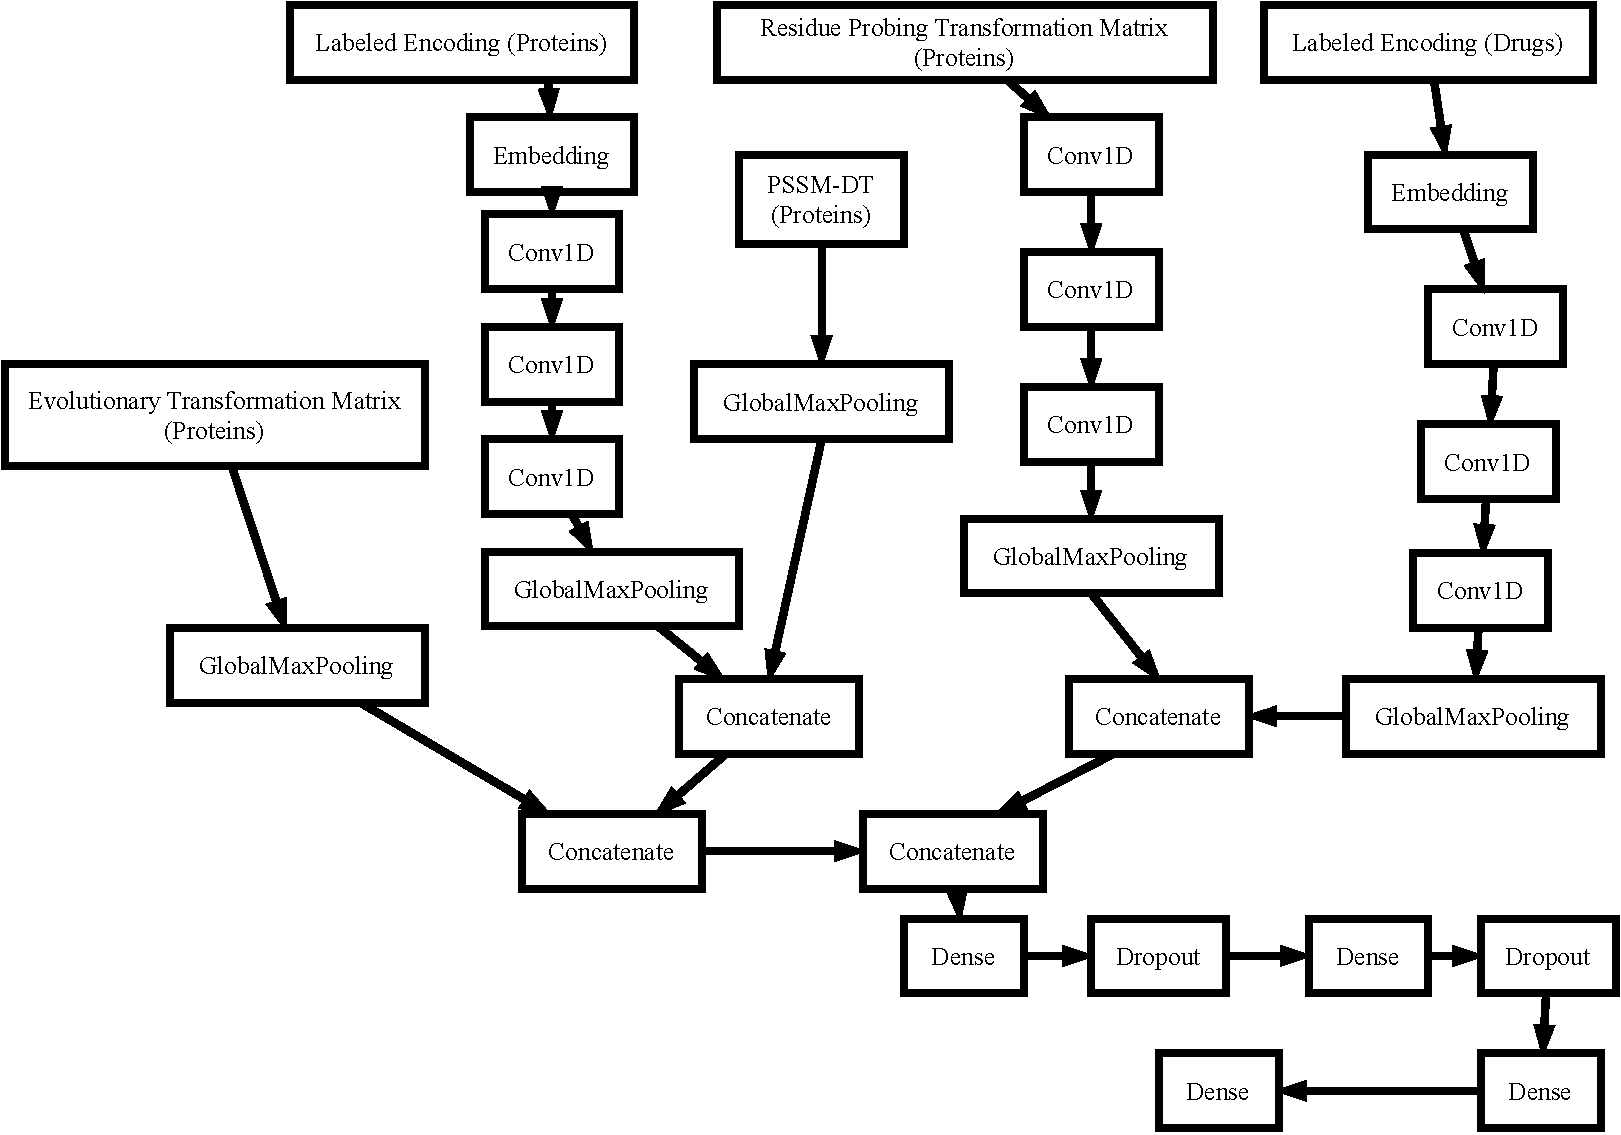
\includegraphics[width=1\linewidth]{mainmatter/3-Methodology/images/DeepDF_monchrome.pdf}
  \caption{Deep Learning Model to predict Protein-Drug Interaction}
  \label{fig:dlm}
  \end{figure}
  \begin{table}[H]\centering
    \caption{Inputs Used in the Deep Learning Network} 
    \begin{tabular}{|l|l|l|l|}
      \hline 
      S.No. & Input Layer Name & Used Feature Vector & Type \\ \hline
      1 & input\_1 & Label Encodings & Drug \\ \hline
      2 & input\_2 & Label Encodings & Protein \\ \hline
      3 & input\_3 & Evolutionary Distance Transformation Vector& Protein \\ \hline
      4 & input\_4 & PSSM-DT Vector & Protein \\ \hline
      5 & input\_5 & Residue Probing Transformation Vector & Protein \\   \hline 
    \end{tabular} 
    \label{table:inputs}
  \end{table}
  
  \subsection{Components description used from Tensorflow (Keras)}
  \subsubsection{Embedding Layer}
  From figure~\ref{fig:dlm}, the Embedding feature provided by keras for vector representation of both drug fingerprint and protein sequence are utilized. The label encodings of the drugs and protein sequences are inputs to this layer. It turns positive integers (indexes) into dense vectors of fixed size. eg. [[4], [20]] -> [[0.25, 0.1], [0.6, -0.2]].
 
  \subsubsection{Convolution Neural Network}
  \acrfull{cnn} are used for feature generation in machine learning system. They improve a machine learning system in three perspectives: sparse interactions, parameter sharing and equivariant representations. While a conventional neural network is tight network for instance, a Dense Layer creates an interaction of every input unit to that of output units; \acrshort{cnn} have sparse interactions. This differentiates the learning pattern of \acrshort{cnn} from other networks by understanding the local patterns in the input vector. While traditional Neural Networks mostly involve learning the global parameters, \acrshort{cnn} is used to learn local patterns. It does so by reducing the kernel (aka filter) smaller than the input. For example, when an image can have thousands of pixels, the kernel size can be tens or hundreds of pixels as shown in Figure ~\ref{fig:cnn}. 
  
  
  \begin{figure}[H]
    \centering
    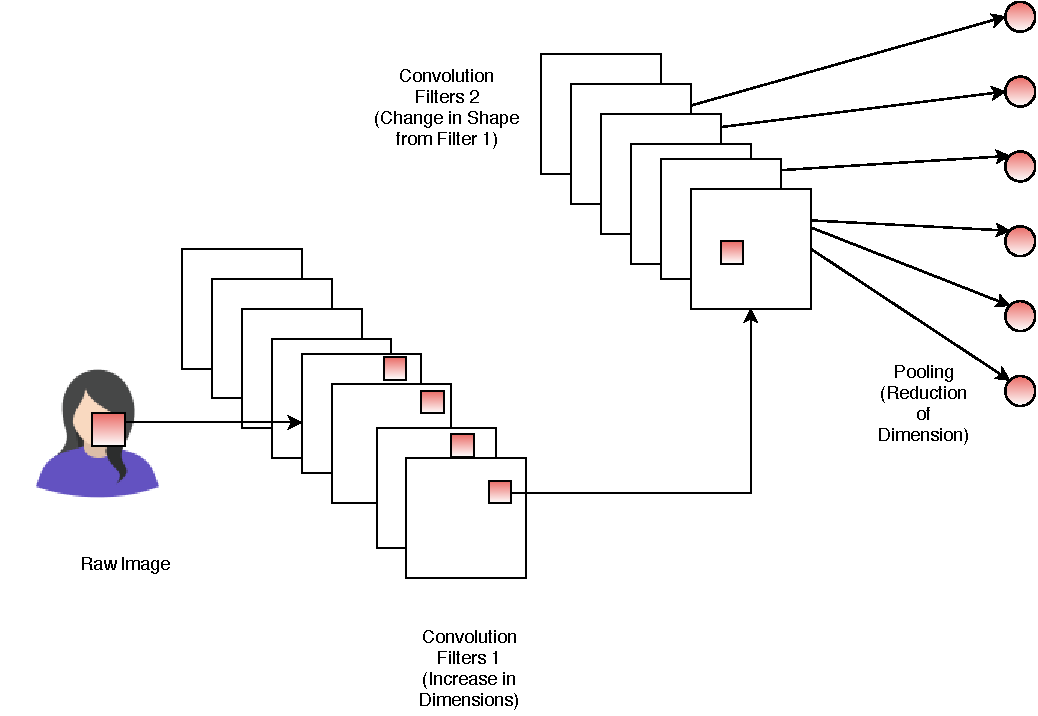
\includegraphics[width=1\linewidth]{mainmatter/3-Methodology/images/System-Block-CNN-Layer.pdf}
    \caption[Working of CNN Block]{Working of CNN Block:The small window from the image grid forms a filter. In first layer there is use of 8 filters}
    \label{fig:cnn}
  \end{figure}
  
  Parameter Sharing refers when the same parameter is used for multiple times in model. In conventional neural net, each parameter is used only once when computing the output of a layer. In \acrshort{cnn}, as the window sweeps over all the images, the same pixels create different representations with the position of sweeping window. So the parameter sharing property of \acrshort{cnn} identifies one representation for the pixel at a time.
  
  Equivariance property of \acrshort{cnn} is caused due to parameter sharing. It is defined as a property defined as when the input is translated, so is the output. When processing some time-series data the convolution produces a timeline sequence of features that appear in the input. For example, the convolution operations in movie will produce the feature timeline for the picture pixels.

  This research uses \acrfull{cnn} to learn the sequential representation of drug and proteins. As the primary structure of proteins and drugs are in fact representations of their 2D representations, the convolution operation will help to learn such features for further analysis. Again, 3D representations are also learned by higher layers of convolution layers. \citep{Adhikari2017}


\iffalse
  \begin{figure}[H]
    \centering
    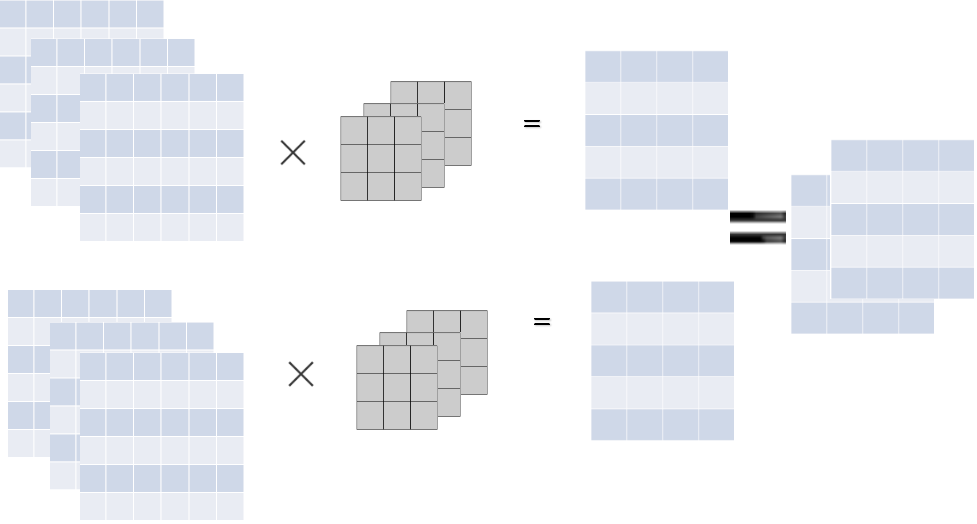
\includegraphics[width=.8\linewidth]{mainmatter/3-Methodology/images/cnn.png}
    \caption{Convolutional Neural Network}
    \label{fig:cnn}
  \end{figure} 
\fi


  
  
  \subsubsection{Pooling Layer}

  \begin{figure}[H] \centering
    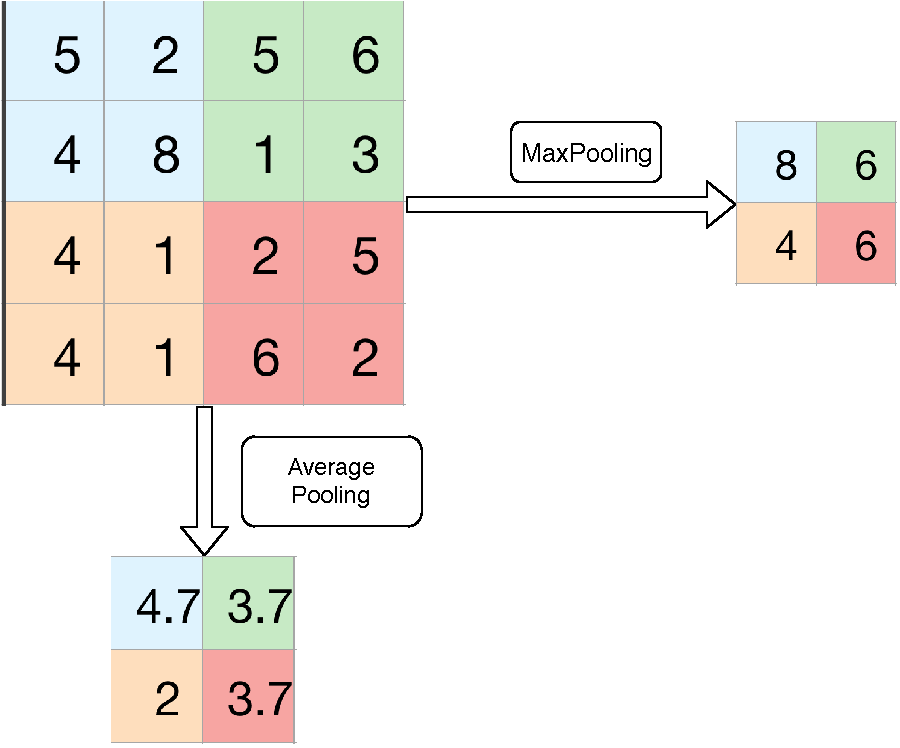
\includegraphics[width=.5\linewidth]{mainmatter/3-Methodology/images/pooling.pdf}
    \caption[Pooling Layer]{Pooling Layer: MaxPooling takes the maximum value from the pooling window and AveragePooling takes the mean from the pooling window.}
    \label{fig:pool_layer}
  \end{figure}

  
  The Pooling layer was used to modify the output of its preceding layer. For example the max pooling renders the maximum output from a rectangular neighborhood and average pooling renders average value from the the rectangular neighborhood. It was used to downsample the learned parameters from the grid of 2 dimensions returned by Convolution Layer. This work used Global Max Pooling to reduce the dimension and extract the extreme features learned from \acrshort{cnn}. Thus, it got reduced to 1 dimension by taking the highest values from the window size(corresponding to shape of 1\textsuperscript{st} dimensional element). The Pooling operation has been described by Figure ~\ref{fig:pool_layer}.

  
  \subsubsection{Dense Layer}
  Dense Layer is a neural layer which fully connects the input layer to output layer. It performs a linear operation on the layer's input vector. At every node in output of the dense layer generally follows an activation function that creates a generalization rule for the input vectors at the node. The research work used the dense layer to learn the global pattern from the feature data. The representation can be seen from Figure ~\ref{fig:dense}. As the output required is a regression value, it uses relu for activation.

  \begin{figure}[ht]
    \centering
    % 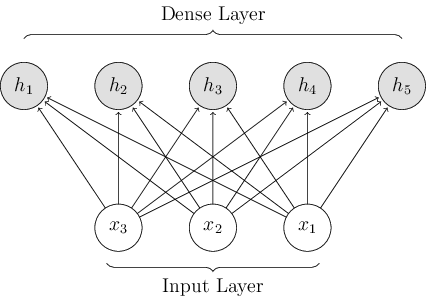
\includegraphics[width=.5\linewidth]{mainmatter/3-Methodology/images/dense.png}
    
  

\begin{tikzpicture}[->,>=stealth',shorten >=1pt,auto,node distance=2.8cm,
    semithick]

      \tikzstyle{every state}=[text=black]
      \node[state]          (A)   {$h_1$};
      \node[state]         (B)  [right of=A] {$h_2$};
      \node[label=above:{Dense Layer},state]         (C) [right of=B] {$h_3$} ;
      \node[state]         (D) [right of=C] {$h_4$};
      \node[state]         (E) [right of=D] {$h_5$};

      \node[state]         (X1) [below of=B] {$x_3$};
      \node[state, label=below:{Input Layer}]         (X2) [right of=X1]       {$x_2$};
      \node[state]         (X3) [right of=X2]       {$x_1$};

      \path (X1) 
      edge              node {} (A)
      edge              node {} (B)
      edge              node {} (C)
      edge              node {} (D)
      edge              node {} (E)
      % edge              node {1,1,R} (C)
      (X2) 
      edge              node {} (A)
      edge              node {} (B)
      edge              node {} (C)
      edge              node {} (D)
      edge              node {} (E)
      % edge              node {0,1,L} (C)
      (X3)
      edge              node {} (A)
      edge              node {} (B)
      edge              node {} (C)
      edge              node {} (D)
      edge              node {} (E);
      % edge [bend left]  node {1,0,R} (E);

\end{tikzpicture}

  
\caption{Dense Layer}
\label{fig:dense}
\end{figure}

  
  \subsubsection{Dropout Layer}
  Our model becomes undesirable when every component of the input layer makes a significant change to the output layer. To reduce the effect of unimportant features the dropout layer was used. Thus the backpropagation network tries to ignore the noise features and minimizes the unrealizable prediction of the learning problem. This has been expressed diagrammatically in Figure ~\ref{fig:dropout}.
  \begin{figure}[tbh] \centering
    \captionsetup{justification=justified}
    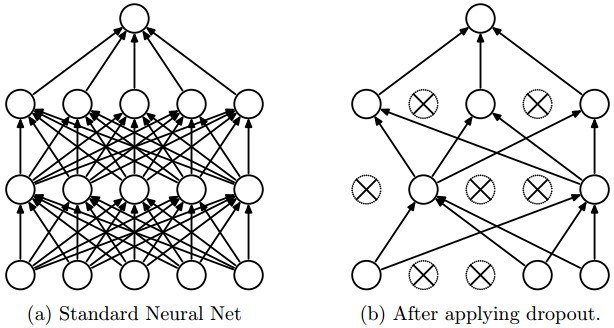
\includegraphics[width=.5\linewidth]{mainmatter/3-Methodology/images/dropout.jpeg}
    \caption[Dropout Layer]{a) Standard neural network whose all the nodes have weights connected to higher nodes and lower nodes. 
    b) Certain nodes belonging to same levels are disconnected. Some weights are also disconnected from other nodes depending on the percentage of dropout applied.}
    \label{fig:dropout}
  
  \end{figure}
  
  
  
  \subsubsection{Concatenation Layer}
  Concatenation Layer as the name implies is used to simply join two vectors so that a feature set comprising of multiple features can be created. Their positional index indicates the feature set being manipulated. The first dimensional length of input matrices and their no. of dimension should be same to concatenate the matrices.

  \subsubsection{Activation Layer}
  
  Activation Layer is a function that takes an input and provides an output based on the value. There are various kinds of Activation functions like Sigmoid, ReLu, Leaky Relu, tanh, Gaussian, Sinusoid etc. The research uses ReLu function for the activation layers.
  
  \subsubsection{Rectified Linear Unit}
  The output of Rectified Linear Unit (ReLu) is from 0 to infinity. For a normalized ReLu, the output will be between 0 to 1. The parametric equation is shown in Eq~\ref{eq:relu}.

  
  \begin{equation}
    f(x) = 
      \begin{cases}
        0 & ,for \quad x <= 0 \\
        x & ,for \quad x > 0
      \end{cases}
      \label{eq:relu}
  \end{equation}

  \begin{figure}
    \centering
    % \subfloat[ Relu Activation ][Relu Activation Function ]{
      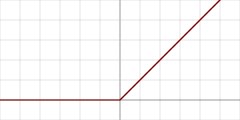
\includegraphics[width=.45\textwidth]{mainmatter/3-Methodology/images/relu.png}
    % }
    \label{fig:relu}
    \caption{Relu Activation Function}
  \end{figure}

   
  \subsection{Choice of Optimizers}

  Optimizers are the functions that estimate the global maximum/minimum for a problem domain. Their characteristics to find the global extremes or local extremes depend on the type of problem type and the optimization parameters used to train the algorithm. The choice of optimizer influences both the speed of convergence and whether it occurs. 
  The optimizers aim to minimize the cost function $ J( \theta; x^{(i)}; y^{(i)}) $ where $\theta$ is the optimization rule for cost function and $x{(i)},y{(i)}$ are the input,output parameters. The optimizers chosen to minimize the cost function associated to protein-drug prediction are:
  
  \subsubsection{Stochastic Gradient Descent(SGD)}

  The optimization formula for \acrfull{sgd}:
  \begin{equation}
    \theta = \theta - \eta \cdot \nabla_\theta J( \theta; x^{(i)}; y^{(i)})
  \end{equation}

  \subsubsection{Adaptive Moment Estimation(Adam)}

  The optimization formula for \acrfull{adam}:
  \begin{equation}
  \begin{aligned} V _ { d \theta } & = \beta _ { 1 } V _ { d \theta } + \left( 1 - \beta _ { 1 } \right) d \theta \\ S _ { d \theta } & = \beta _ { 2 } S _ { d \theta } + \left( 1 - \beta _ { 2 } \right) d \theta \\ V \operatorname { corr } _ { d \theta } & = \frac { V _ { d \theta } } { \left( 1 - \beta _ { 1 } \right) ^ { t } } \\ S c o r r _ { d \theta } & = \frac { S _ { d \theta } } { \left( 1 - \beta _ { 2 } \right) ^ { t } } \\ \theta & = \theta - \alpha \frac { d \theta } { \sqrt { S _ { d \theta } } + \varepsilon } \end{aligned}
  \end{equation}

  \subsubsection{Root Mean Squared Propagation(RMSProp)}

  \begin{equation}
    W_{dW} = \beta{W_{dW}} + (1-\beta) {\nabla\theta}^{2}
  \end{equation}

  \begin{equation}
    \theta = \theta - \eta \cdot \frac{\nabla_\theta}{\sqrt{W_{dW}} + \epsilon}  J( \theta; x^{(i)}; y^{(i)})
  \end{equation}


  \subsubsection{Adaptive Gradient Algorithm(AdaGrad)}
  
  \begin{equation}
    W_{dW} = \beta{W_{dW}} + (1-\beta) {\nabla\theta}
  \end{equation}

  \begin{equation}
    \theta = \theta - \eta \cdot W_{dW} J( \theta; x^{(i)}; y^{(i)})
  \end{equation}


  
  \iffalse
  \subsubsection{LSTM}
  As the \acrfull{rnn} often suffers from vanishing gradient problem~\footnote{Vanishing Gradient:During the training of RNN, the model vectors form a part of a loop and makes an unstable network.}, we use a \acrshort{lstm} Layer to learn the global pattern of the feature sets resulting after concatenation of different stacked layers outputs. The LSTM architecture can be seen in Figure ~\ref{fig:lstm}:
  \begin{figure} 
    [t]
    \centering
    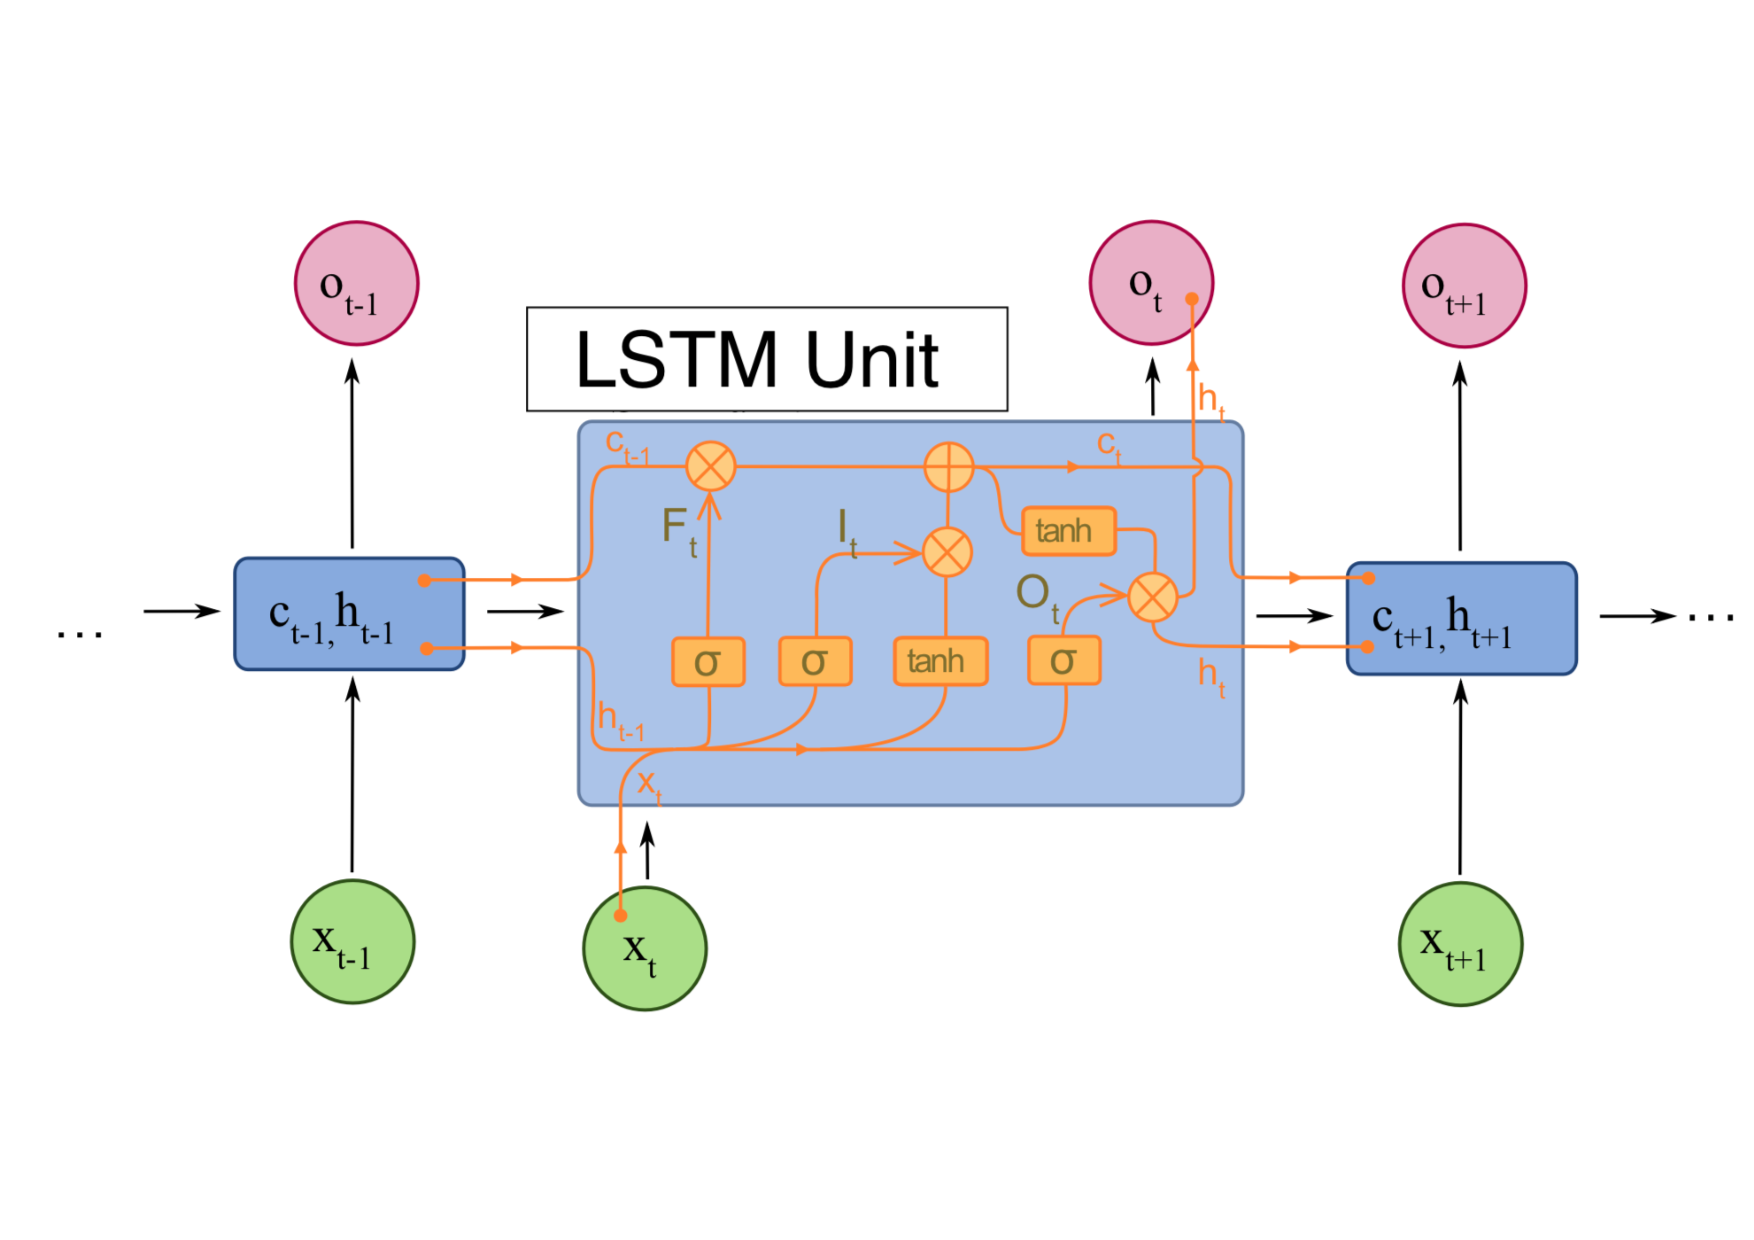
\includegraphics[width=1\linewidth]{mainmatter/3-Methodology/images/LSTM.pdf}
    \caption{Long Short Term Memory}
    \label{fig:lstm}
  \end{figure}
  In Figure~\ref{fig:lstm}, we can see that it contains a forget node, memory node and output node. These three nodes balance the information that needs to be removed, stored for future updates and necessarily fire the output node to make correct prediction.
  \fi
\chapter{Experiments and Results}


\section{Experiments}

\iffalse
SVM-Regression
Random-Forest Regression
Deep Learning Network

Neural Net Sequence Embeddings
One-Hot Encodings
Modfied n-grams skip-grams
\fi

The focus of the experiments are concentrated on the properties of protein as they have complex structures. The binding of protein and drug depend on various attributes of protein like acidity, hydrophobicity, binding pockets etc and the structure of drug. The attributes are quite closely related to primary and secondary structure of protein themselves. Therefore, our model aims to relate all these multiple components with matrix representation and confirming to the Figure.~\ref{fig:kiba_drug_protein} prediction.

\subsection{Features Selection}
\subsubsection{Primary Feature Selection}
We explored the other embedding technique used in language theory. The modified N-Grams Skip-Grams (m-NGSG) was supposed to undertake the mutational agreements when the proteins and drug interaction was brought in question. However, it fared quite badly than the Neural Net Sequence Embeddings. Mostly the issue can be related to that if the algorithm misses the tight relationship among the amino-acid neighborhood, then the protein with different structure may seem to act similarly: a strong disagreement on principle that certain proteins with slight modification on the sequence have different functional and chemical properties. It could still be used for Poission-Hidden Markov Model for some other properties, but primary encodings can't be relied on m-NGSG. 

Therefore we relied on Neural Net Sequence Embedding technique to form the primary representation. Both protein and drug were converted to Embedding vectors after creating their one-hot encoding.

\subsubsection{Secondary Features Selection}
These are the structural components of protein especially related to alpha and beta strands of Protein segments. All the protein Sequences are subjected to Equation~(\ref{eq:pssm}) from the one-hot encodings. The \acrshort{pssm} matrix is calculated using PSI-BLAST\cite{Schaffer2001}. Then all the testing protein sets are evaluated with the resultant PSSM to form a new PSSM matrix specific to the testing protein. Thus, we expect to explore how proteins relate with the interaction experiments with the protein domain. From the \acrshort{pssm}, we evaluate the other evolutionary and distance vectors using equations \ref{eq:rpt}, \ref{eq:pssmddt}, \ref{eq:pssmsdt} and \ref{eq:edt}.

\subsection{Implementation}
% We explore basically the following algorithms for analyses on protein-drug interactions:

\subsubsection{Stacked Features, LSTM Network}
Basically, we implement the ~\ref{fig:dlm} for our model design. It is implemented in Python using the TensorFlow framework consisting of keras. The training contained of 100 epochs and required full 4 complete days to complete the training in a high GPU processors. The training and testing was done in a 5-fold cross-validation set prepared manually. To evaluate the performance of the model, we used concordance index(CI)\cite{Xu2015} as defined by equation~\ref{eq:ci}:
\begin{equation}
    CI = \frac{1}{Z} \sum_{\delta_i > \delta_j} h(b_i - b_j)
    \label{eq:ci}
\end{equation}
where $b_i$ is the prediction value for higher affinity $\delta_i$ and $b_j$ is the prediction value for smallery affinity $\delta_j$, $Z$ is the normalization constant and $h(m)$ is the unit step function:
\begin{equation} h(x) = 
    \begin{cases}
        1,& \quad {if x>0} \\
        0.5, & \quad{ if x=0 } \\
        0, & \quad{if x<0} \\
    \end{cases}
\end{equation}

\section{Results}
The validation loss and the cindex scores were 16\% and 90\% respectively when we used our full model. 

\iffalse
The accuracy plots and cindex plots are shown in Figure ~\ref{fig:results}
\begin{figure}
    
\end{figure}
\fi
\chapter{Conclusions}

The research was conducted for series of experiments using different CNN architectures and validated using four different settings of drug and protein combinations. The experiments show that the network requires past knowledge on proteins and drugs to yield the best results. The model could yield best scores when both the protein and drug were present in the training phase. We also conclude that if the domain has fewer parameters to learn from, we can represent them in new dimensions to achieve better results in machine learning problem.

Finally, it concludes that:
\begin{itemize}
    \item Proteins need to be represented in higher dimensions of R2RSRV factors and the domain representation by using PSSM features along with the sequence information for formulating protein-solving network architecture.
    \item Same filter size of 8 can be used to train the CNN layer for both proteins and drugs.
\end{itemize}

\chapter{Recommendations}
% \section{Future Works}

At present, the sample space of~\acrfull{nfl} has been explored by forming the different feature-sets. The different feature sets on chemical values of drugs can be used to represent a much broader spectrum of drug molecule representation. In case of protein, protein folds could be the incorporated information which could be supplemented for the available 3D protein structures and a good prediction algorithm chosen for CASP\citep{CASP82008}. For the features being evaluated, the Grid-Search CV could be applied over various algorithms and Stacking Generalization could be used to create a better optimized machine learning solution to predict protein-drug interaction score from sequence information. Successively, important is a correct modeling of Pharmacophore modeling of drug-proteins pairs so that it can be applied directly to medical supervisions. 



% Backmatter

\begin{landscape}
\appendix
\chapter*{Appendix A: R2RSRV}
\begin{table}[H]
    \centering
    \small  
    \setlength{\tabcolsep}{1pt}\iffalse
    \begin{tabular}{p{.8cm}p{.8cm}p{.8cm}p{.8cm}p{.8cm}p{.8cm}p{.8cm}p{.8cm}p{.8cm}p{.8cm}p{.8cm}p{.8cm}p{.8cm}p{.8cm}p{.8cm}p{.8cm}p{.8cm}p{.8cm}p{.8cm}p{.8cm}p{.8cm}}
        \fi \caption[]{R2RSRV Matrix}
        \begin{tabular}{|c|c|c|c|c|c|c|c|c|c|c|c|c|c|c|c|c|c|c|c|c|}
            \hline
            &I&V&L&F&C&M&A&G&T&S&W&Y&P&H&E&Q&D&N&K&R\\ \toprule \hline
            I&5.21&2.42&0.88&1.71&-1.59&1.13&0.95&0.48&-1.05&-3.20&0.65&1.44&-0.82&-1.54&-0.94&-0.62&-1.66&-3.14&-2.23&-2.14\\ \hline
            V&2.42&9.46&1.33&0.49&-0.32&0.54&1.55&-2.12&-0.91&-1.80&-2.88&-1.05&-0.81&-1.32&-0.29&-0.58&-2.39&-3.69&0.66&-1.42\\ \hline
            L&0.88&1.33&9.90&1.08&-0.42&2.17&2.41&-2.29&-3.40&-2.32&0.48&-0.77&-2.28&1.67&-0.77&-0.08&-3.49&-2.16&-2.10&0.19\\ \hline
            F&1.71&0.49&1.05&6.11&0.55&0.89&0.52&-2.00&-1.10&-2.09&-0.11&1.14&0.83&-1.33&-1.79&0.42&-3.62&-0.96&-1.71&-1.33\\ \hline
            C&-1.59&-32&-0.42&0.55&15.35&-1.35&-0.21&0.59&-1.52&1.53&-1.07&-1.16&0.28&0.95&-0.52&-1.47&-1.95&-2.23&-1.80&-0.84\\ \hline
            M&1.13&0.54&2.17&0.89&-1.35&5.40&-0.28&0.44&-2.15&-1.50&-0.71&-0.33&-0.31&0.19&0.01&0.27&-3.38&-1.74&-0.72&-1.51\\ \hline
            A&0.95&1.55&2.41&0.52&-0.21&-0.28&7.08&-2.04&-1.04&-0.61&-1.15&-1.22&-1.58&0.11&-0.53&-0.82&-1.06&0.17&-1.11&-2.74\\ \hline
            G&0.48&-2.12&-2.29&-2.00&0.59&0.44&-2.04&5.65&1.67&-1.32&-0.82&0.27&-0.60&0.75&-2.24&1.68&0.70&-1.01&1.72&1.22\\ \hline
            T&-1.05&-0.91&-3.40&-1.10&-1.52&-2.15&-1.04&1.67&4.42&1.23&0.59&-1.36&-0.04&-1.48&-0.06&-2.61&4.66&0.02&0.29&-0.74\\ \hline
            S&-3.20&-1.80&-2.32&-2.09&1.53&-1.50&-0.61&-1.32&1.23&6.22&-1.10&-1.40&-0.79&-2.66&2.14&-0.08&4.57&0.95&0.11&-0.38\\ \hline
            W&0.65&-2.88&0.48&-0.11&-1.07&-0.71&-1.15&-0.82&0.59&-1.10&1.08&-0.45&5.88&0.15&-2.84&-2.84&-1.98&-1.35&-0.27&4.08\\ \hline
            Y&1.44&-1.05&-0.77&1.14&-1.16&-0.33&-1.22&0.27&-1.36&-1.40&-0.45&6.40&0.21&1.11&0.75&-2.73&-3.07&-0.45&0.87&-0.33\\ \hline
            P&-0.82&-0.81&-2.28&0.83&0.28&-0.31&-1.58&-0.60&-0.04&-0.79&5.88&0.21&1.73&-1.13&0.66&0.82&-2.51&1.37&0.14&-0.40\\ \hline
            H&-1.54&-1.32&1.67&-1.33&0.95&0.19&0.11&0.75&-1.48&-2.66&0.15&1.11&-1.13&5.03&-2.22&0.32&3.11&-1.46&-1.90&-0.06\\ \hline
            E&-0.94&-0.29&-0.77&-1.79&-0.52&0.01&-0.53&-2.24&-0.06&2.14&-2.84&0.75&0.66&-2.22&2.59&-1.98&-4.29&0.07&3.52&3.45\\ \hline
            Q&-0.62&-0.58&-0.08&0.42&-1.47&0.27&-0.82&1.68&-2.61&-0.08&-2.84&-2.73&0.82&0.32&-1.98&3.44&0.79&0.92&-0.67&0.24\\ \hline
            D&-1.66&-2.39&-3.49&-3.62&-1.95&-3.38&-1.06&0.70&4.66&4.57&-1.98&-3.07&-2.51&3.11&-4.29&0.79&1.69&3.85&0.86&2.73\\ \hline
            N&-3.14&-3.69&-2.16&-0.96&-2.23&-1.74&0.17&-1.01&0.02&0.95&-1.35&-0.45&1.37&-1.46&0.07&0.92&3.85&7.91&-0.63&-0.43\\ \hline
            K&-2.23&0.66&-2.10&-1.71&-1.80&-0.72&-1.11&1.72&0.29&0.11&-0.27&0.87&0.14&-1.90&3.52&-0.67&0.86&-0.63&2.61&-3.54\\ \hline
            R&-2.14&-1.42&0.19&-1.33&-0.84&-1.51&-2.74&1.22&-0.74&-0.38&4.08&-0.33&-0.40&-0.06&3.45&0.24&2.73&-0.43&-3.54&0.73 \\ \hline
        
    \end{tabular}
    \label{table:r2r}
\end{table}
\end{landscape}

    
\printglossary[type=\acronymtype]

% Bibliography
\bibliographystyle{unsrt}
\bibliography{bibliography/sample}
\addcontentsline{toc}{chapter}{Bibliography}



\end{document}

%%%%%%%%%%%%%%%%% END OF MAIN DOCUMENT
